\documentclass[12pt, a4paper]{article}

% ===== PACKAGES =====
\usepackage[utf8]{inputenc}
\usepackage[a4paper,total={170mm,257mm},left=20mm,top=20mm,right=20mm,bottom=25mm,headheight=14.5pt]{geometry}
\usepackage{graphicx}
\graphicspath{{figures/}}
\usepackage{amsmath,amssymb,amsthm,mathtools}
\usepackage{bm}
\usepackage{booktabs}
\usepackage{tabularx}
\usepackage{array}
\usepackage{hyperref}
\usepackage{xcolor}
\usepackage{caption}
\usepackage{subcaption}
\usepackage{titlesec}
\usepackage{enumitem}
\usepackage{times}

\hypersetup{colorlinks=true,linkcolor=blue!50!black,citecolor=green!50!black,
  urlcolor=red!50!black,pdftitle={PDM: Unsupervised Anomaly Detection in Pediatric Brain MRI},
  pdfauthor={Soham Patel}}

\allowdisplaybreaks
\setlength{\jot}{5pt}

% theorem environments + macros required by the appended derivation (math_body.tex)
\newtheorem{theorem}{Theorem}
\newtheorem{proposition}{Proposition}
\newtheorem{lemma}{Lemma}
\theoremstyle{definition}\newtheorem{definition}{Definition}
\newcommand{\R}{\mathbb{R}}
\newcommand{\E}{\mathbb{E}}
\newcommand{\N}{\mathcal{N}}
\newcommand{\KL}{\mathrm{D_{KL}}}
\newcommand{\x}{\bm{x}}
\newcommand{\z}{\bm{z}}
\newcommand{\eps}{\bm{\epsilon}}
\newcommand{\II}{\mathbf{I}}
\newcommand{\abar}{\bar{\alpha}}
\newcommand{\given}{\,\vert\,}
\DeclareMathOperator*{\argmin}{arg\,min}
\DeclareMathOperator*{\argmax}{arg\,max}
\DeclareMathOperator{\ReLU}{ReLU}
\DeclareMathOperator{\Var}{Var}

\titleformat{\section}{\normalfont\Large\bfseries\color{black!80}}{\thesection}{1em}{}
\titleformat{\subsection}{\normalfont\large\bfseries\color{black!75}}{\thesubsection}{1em}{}
\titleformat{\subsubsection}{\normalfont\normalsize\bfseries\color{black!70}}{\thesubsubsection}{1em}{}
\captionsetup{labelfont=bf,textfont=it,justification=raggedright,singlelinecheck=false}

\begin{document}

% ===== TITLE PAGE =====
\begin{titlepage}
  \begin{center}
    \vspace*{1.5cm}
    {\Huge\bfseries Project Report}\\[1.2cm]
    \includegraphics[width=9cm]{oth.png}\\[1.2cm]
    {\Large\bfseries ``Deep Vision (Summer 2025)''}\\[0.8cm]
    {\large\itshape Patch-Diffusion Models for Unsupervised, Explainable\\
      Anomaly Detection in Pediatric Brain MRI}\\[1.6cm]
    {\small\bfseries Submitted by}\\[0.2cm]{\Large\bfseries Soham Patel}\\[0.9cm]
    {\small\bfseries Supervised by}\\[0.2cm]{\Large\bfseries [Supervisor Name]}\\[1.6cm]
    \begin{center}
      {\small Ostbayerische Technische Hochschule Amberg-Weiden}\\
      {\small Department of Electrical Engineering, Media and Computer Science}
    \end{center}
    \vfill {\large\today}
  \end{center}
\end{titlepage}

\pagenumbering{roman}
{\small\tableofcontents}
\clearpage

% ===== ABSTRACT =====
\thispagestyle{empty}
\vspace*{\fill}
\begin{center}\begin{minipage}{0.86\textwidth}
\section*{Abstract}
This report presents a \textbf{pixel-space patch-diffusion model (PDM)} for
\textbf{unsupervised anomaly detection (UAD)} in pediatric brain MRI, trained on the
BraTS-PEDs cohort with \textbf{no lesion labels}. A four-channel denoising diffusion model
(25.3\,M-parameter U-Net) learns the distribution of \emph{healthy} $96{\times}96$
image patches under spatially-correlated (simplex) noise. At inference, a test slice
is partially noised and then denoised with DDIM back toward the healthy manifold, and
the multi-scale, modality-weighted reconstruction residual localises the pathology.
The healthy reconstruction is itself a faithful \emph{counterfactual}, complemented by
exact per-modality and per-scale residual attribution. The experiments use a
deliberately small \textbf{30-patient pilot} (60 epochs, one NVIDIA A100 80\,GB), drawn
from a full BraTS-PEDs split that was preprocessed but not fully used here for reasons
of time and compute (\S\ref{sec:pilot}). The diffusion model trains well, reaching a
best validation noise-MSE of \textbf{0.0604} (about 94\% of the injected-noise variance
explained). Over 204 evaluated test slices the system attains
\textbf{AUROC $=0.713$}, \textbf{AUPRC $=0.076$}, calibrated \textbf{Dice $=0.076$}
(oracle Dice $0.138$). On its best-represented patient it reaches AUROC $0.96$ and slice
Dice up to $0.58$ --- in the range of methods trained on full adult cohorts, although
that comparison is limited by different datasets, supervision levels and evaluation
protocols. The average Dice of $0.076$ is clearly below published results
($0.24$--$0.60$), and with only four test patients statistically reliable conclusions
are not possible. The failure analysis points to a most likely cause: patient-level
reconstruction fidelity. When a patient's anatomy is poorly represented in training, the
residual is high almost everywhere and the lesion can no longer be separated
(AUROC $<0.5$). On slices where the score does separate the two classes, the calibrated
threshold is already near-optimal (within $0.005$ Dice of the sweep optimum). The most
plausible limiting factor is therefore training-set size rather than the detector design,
a hypothesis stated carefully given the small sample.
\end{minipage}\end{center}
\vspace*{\fill}\clearpage

\pagenumbering{arabic}

% =====================================================================
\section{Introduction}
% =====================================================================
Detecting tumours in brain MRI is usually posed as \emph{supervised}
segmentation. That approach needs large sets of expert voxel annotations and, by
design, only learns the pathologies that appear in the training labels.
\textbf{Unsupervised anomaly detection (UAD)} turns the problem around: a generative
model learns the distribution of \emph{healthy} anatomy, and any large enough
deviation from it is flagged as anomalous \cite{baur2021,schlegl2019}. This removes the
annotation bottleneck \emph{at training time} (expert masks are still needed at
evaluation time to measure accuracy), and the detector is in principle agnostic to the
lesion type, because it responds to any departure from normality.

This matters especially in the \textbf{pediatric} setting. Models trained on adults
do not transfer cleanly to children for several reasons: the developing brain changes
appearance with age as myelination progresses; pediatric tumours are histologically
different from adult ones (for example DIPG/DMG rather than adult glioblastoma); the
smaller head changes the spatial scale of structures; and edema patterns differ. On
top of this, labelled pediatric data are scarce \cite{kazerooni2024}. A method that
learns only from healthy anatomy is therefore an attractive fit.

Denoising diffusion probabilistic models (DDPMs) \cite{ho2020} have become a popular
backbone for reconstruction-based UAD \cite{wyatt2022,behrendt2023}. A model trained
only on healthy data, when asked to denoise a corrupted pathological image, tends to
fill the abnormal region with the most probable healthy continuation, so the lesion
survives as a reconstruction residual. This work designs, trains and critically
evaluates such a system for pediatric brain MRI. Its main contribution is not a new
component but an honest, leakage-controlled study of \emph{when and why} the method
succeeds or fails. It should be noted up front that inference is slow (about 92\,s per
slice, \S\ref{sec:setup}), so the current system is a research prototype rather than a
clinically deployable tool.

\subsection{Problem statement and objectives}
Given an unseen multi-modal MRI slice, produce a per-pixel anomaly map (and a
binary lesion prediction) using a model trained \emph{only} on lesion-free anatomy.
Objectives: (a) learn a healthy-manifold diffusion model over multi-modal MRI
patches; (b) convert reconstruction residuals into a calibrated, label-free anomaly
score; (c) explain inference behaviour with faithful, decision-intrinsic
explainers (counterfactual generation and exact residual attribution); (d) quantify
performance with AUROC/AUPRC/Dice and compare
against the literature; and (e) diagnose the dominant failure mode with
figure-backed, leakage-proof evidence and propose a concrete fix.

% =====================================================================
\section{Related Work}
% =====================================================================
\subsection{Autoencoder- and GAN-based methods}
The earliest reconstruction-based UAD methods learn a healthy model $g$ and score a
test image by its reconstruction residual $\|\x-g(\x)\|$. Convolutional and variational
autoencoders were compared systematically by Baur et al. \cite{baur2021}; f-AnoGAN
\cite{schlegl2019} replaces the decoder with a GAN generator and adds a
discriminator-feature term. (The f-AnoGAN Dice of about $0.24$ quoted later is from
Baur et al.'s unified re-implementation, not the original paper, which used a different
setup.) All of these share one recurring weakness, the \emph{identity shortcut}: a model
expressive enough to reconstruct healthy tissue well often reconstructs the lesion too,
which collapses the residual.

\subsection{Diffusion-based methods}
Diffusion models reduce the identity-shortcut problem because the amount of injected
noise can be tuned to erase a localised lesion while keeping the global anatomy.
AnoDDPM \cite{wyatt2022} introduced \emph{partial}-noise reconstruction and
\textbf{simplex (correlated) noise}, which corrupts the mid-to-large spatial scale of
lesions rather than fine pixel detail. pDDPM \cite{behrendt2023} reconstructs in
overlapping \emph{patches} to improve healthy-tissue fidelity. Wolleb et al.
\cite{wolleb2022} use DDIM sampling with classifier guidance and report Dice around
$0.60$ on adult BraTS; this is the closest method in machinery to the present one (it
also uses DDIM on BraTS), but it is \emph{weakly supervised}, whereas this work uses no
labels at
all. Pinaya et al. \cite{pinaya2022} run the same idea in the \emph{latent} space of a
VAE for speed --- the design point this project deliberately moves away from
(\S\ref{sec:approach}). Bercea et al. \cite{bercea2023} both propose multi-noise-level
scoring and, importantly, show that many UAD methods are biased toward bright
(hyperintense) FLAIR lesions; this critique directly motivates the explicit modality
weighting used here (\S\ref{sec:approach}).
Reporting Dice at calibrated, best-global and oracle thresholds is standard practice,
because the gap between them shows how much performance is lost to thresholding
\cite{zimmerer2022,baur2021}.

\subsection{Positioning of this work}
This project combines partial-noise DDIM reconstruction, simplex noise, patch-wise
diffusion with Gaussian fusion, multi-scale scoring, and a modality-weighted
contrast-enhancement residual into one pipeline, together with a
\emph{counterfactual-first} explainability layer. No individual component is novel. The
contribution is putting them together and then testing carefully when and why the result
works --- including an honest analysis of where it fails (\S\ref{sec:failure}).

% =====================================================================
\section{Approach and Justification}
\label{sec:approach}
% =====================================================================
This section explains each design choice and the reasoning behind it.

\paragraph{Pixel-space, not latent, diffusion.}
An earlier version of this project ran diffusion in the latent space of a
4-channel medical KL-VAE (the standard latent-diffusion recipe, as in Pinaya et al.
\cite{pinaya2022}). That pilot detected lesions well (slice AUROC $\approx0.86$--$0.94$)
but produced an almost unusable segmentation (calibrated Dice $\approx0.00$--$0.10$). The
problem traced back to the VAE: an $\times8$ autoencoder under-reconstructs the sharp
brain/background boundary, which creates a large, roughly constant residual ring around
the whole brain. A single global threshold then cannot separate that ring from the real
lesion. Moving to \emph{pixel}-space patch diffusion removes the VAE entirely, so the
residual is computed directly in interpretable image space and the boundary ring
disappears at its source. (This is a summary of the transition; the full analysis is in
a companion note.)

\paragraph{Patch diffusion \cite{behrendt2023}.}
Each $256{\times}256$ slice is tiled into overlapping $96{\times}96$ patches with stride
$16$. With this geometry each axis yields $\lfloor(256-96)/16\rfloor+1=11$ positions,
so a slice produces $11\times11=121$ patches. The 30-patient pilot pool contains roughly
$3{,}000$ healthy slices, which gives on the order of $3{,}000\times121\approx360{,}000$
training patches (about $120\times$ data amplification; the per-epoch loader then samples
a 250k subset, \S\ref{sec:setup}). This amplification is what makes training viable in
the low-patient pediatric regime, and patching also forces the model to learn
\emph{local} texture rather than memorising whole-slice layout.

\paragraph{Patch size $96{\times}96$ (larger than pDDPM).}
The original pDDPM \cite{behrendt2023} used $48{\times}48$--$64{\times}64$ patches with
stride equal to the patch size (no overlap). The larger $96{\times}96$ patches with
a small stride of $16$ (heavy overlap) were chosen for two reasons: a larger patch gives
the model enough anatomical context to tell normal pediatric structures apart from
lesions, and the heavy overlap lets the Gaussian fusion (\S\ref{sec:method}) average many
predictions per pixel, which suppresses patch-edge artefacts. This is a deliberate
departure from pDDPM rather than an oversight; no controlled ablation of patch size was
run, however, so it is reported as a design choice rather than an optimised one.

\paragraph{Simplex noise \cite{wyatt2022}.}
Simplex noise is dominated by low spatial frequencies, so it corrupts blob-like tumours
at their own scale and the model heals them well (\S\ref{sec:method},
Fig.~\ref{fig:schedule}). This benefit is task-dependent, however: Kascenas et al.
\cite{kascenas2023} find that simplex noise helps for compact, hyperintense tumours but
can hurt for other anomaly types. Its use here is appropriate for BraTS-PEDs tumours but
may not generalise to all anomalies.

\paragraph{Multi-scale scoring \cite{bercea2023}.}
Scoring at three noise levels $T\in\{50,150,250\}$ covers fine, high-SNR anomalies up to
large, low-SNR structural ones. These three values were chosen by hand to span the
schedule (their SNRs are $+20.8$, $+11.9$ and $+7.4$\,dB; Fig.~\ref{fig:schedule}), not
by a grid search; the weighting that combines them was also set by hand.

\paragraph{Modality weighting and the CE channel \cite{menze2015}.}
FLAIR (edema) and contrast enhancement ($t1c-t1n$) carry most of the tumour signal, so
they are up-weighted. These weights are heuristic, based on radiological salience, and
were not optimised or ablated; this is flagged clearly in §\ref{sec:future}.

\paragraph{Counterfactual-first explainability \cite{wachter2017,sanchez2022,wolleb2022}.}
The healthy reconstruction \emph{is} the decision variable, so the difference
$|\x-\hat\x|$ is a faithful explanation by construction. Post-hoc saliency (Grad-CAM) is
deliberately rejected, as it is unfaithful for a generative denoiser
\cite{adebayo2018,rudin2019} (\S\ref{sec:xai}).

% =====================================================================
\section{Data, MRI Modalities and Preprocessing}
% =====================================================================
\subsection{Dataset and the four MRI modalities}
The dataset is \textbf{BraTS-PEDs} \cite{kazerooni2024}, in which each patient provides
four co-registered, skull-stripped MRI modalities and an expert tumour segmentation used
\emph{only for evaluation}. The modalities are physically complementary:
\begin{itemize}[leftmargin=1.3em,itemsep=1pt]
\item \textbf{T1 native ($t1n$)} --- anatomical reference; fluids dark, fat/white-matter bright.
\item \textbf{T1 contrast-enhanced ($t1c$)} --- gadolinium highlights blood-brain-barrier
breakdown, marking \emph{active} tumour.
\item \textbf{T2-weighted ($t2w$)} --- fluids bright; reveals edema and cystic components.
\item \textbf{T2-FLAIR ($t2f$)} --- T2 with CSF suppressed; the most sensitive to
peritumoural edema and infiltration.
\end{itemize}
No single modality captures a tumour: enhancement is a $t1c$ phenomenon, edema a
$t2f/t2w$ one. All four are therefore kept, plus an explicit
\textbf{contrast-enhancement (CE) residual channel} $t1c-t1n$ \cite{menze2015}. The CE
channel assumes that $t1c$ and $t1n$ are well co-registered; BraTS-PEDs provides this,
but raw clinical data might not, in which case the CE term would need a registration
step first.

\paragraph{How one model processes all four modalities jointly.}
The four modalities are stacked into a single global \textbf{4-channel slice
tensor} $\x_{\text{slice}}\in\R^{4\times256\times256}$, from which the
$96{\times}96$ training/inference patches $\x\in\R^{4\times96\times96}$ are
subsequently extracted (\S\ref{sec:method}). The diffusion U-Net operates on these
4-channel \emph{patches} with \texttt{in\_channels}=\texttt{out\_channels}=4, so the
very first convolution mixes the four modalities at every spatial location and
\emph{all} subsequent features are jointly modality-aware; the network predicts a
4-channel noise tensor $\eps_\theta$ in one forward pass. The four modalities are thus denoised \emph{coherently} (a structure
must be explained consistently across modalities to be reconstructed), and the
\emph{score} re-weights the per-channel residuals by clinical salience plus the CE
channel (\S\ref{sec:method}). This is strictly richer than per-modality models,
which cannot exploit cross-modal consistency.

\subsection{Preprocessing and its justification}
(i) \textbf{Axial slicing} to $256{\times}256$. (ii) \textbf{Robust intensity
normalisation} per modality to $[-1,1]$ using the $[0.5,99.5]$ percentile clip
rather than $\pm3\sigma$ --- the latter truncates exactly the FLAIR/enhancement
hyper-intensities that carry the lesion signal. (iii) \textbf{Healthy-pool
construction}: a slice enters diffusion training only if it is lesion-free \emph{and}
at least $3$ slices away from any lesion, which prevents partial-volume tumour tissue
from leaking into the healthy manifold. This filtering uses lesion masks and so applies
only to the training and validation patients; test patients are never filtered this way
and are evaluated on all of their lesion slices. (iv) \textbf{Patch extraction}:
overlapping $96{\times}96$ patches, stride $16$, keeping only patches with foreground
fraction $\ge0.10$.

\subsection{Data-leakage prevention (keeping the evaluation honest)}
\label{sec:leakage}
Every result in this report is protected against optimistic bias by four explicit
controls, so the reported metrics neither over- nor under-state the method:
\begin{enumerate}[leftmargin=1.5em,itemsep=1pt]
\item \textbf{Patient-level disjoint splits.} Train/validation/test are partitioned
by \emph{patient ID}; no slice of a test patient is ever seen in training or
calibration. This rules out the most common medical-imaging leak (adjacent slices
of one patient straddling the split).
\item \textbf{Label-free training.} The diffusion model and the VAE-free residual
use \emph{no} segmentation masks; masks appear only in the final metric computation.
There is therefore no path for label information to enter the model.
\item \textbf{Healthy-only manifold + buffer.} The $\ge3$-slice lesion buffer
prevents tumour-adjacent tissue from contaminating the healthy distribution, so the
model cannot ``learn the lesion'' and then trivially reconstruct it.
\item \textbf{Calibration on held-out healthy slices.} The operating threshold
$\tau$ is fit on healthy validation slices only (\S\ref{sec:method}); it never sees
test data or any lesion.
\end{enumerate}
Consequently the strong result on patient P00002 is \emph{not} leakage, and the
weak result on P00216 is \emph{not} an artefact of an unfair split --- both are
genuine generalisation behaviour on unseen patients (\S\ref{sec:failure}).

\subsection{Dataset scale and why this is a pilot}
\label{sec:pilot}
The full BraTS-PEDs split used here was preprocessed into a patient-disjoint
train/validation/test partition of \textbf{180 / 39 / 38 patients} (about $25{,}000$
healthy slices and $13{,}500$ lesion slices in total). The experiments in this report,
however, deliberately use only a small part of that: \textbf{30 training patients} and
\textbf{4 test patients} (204 lesion slices). This is a pilot, and the reason is
practical rather than methodological. The project ran on a 30-day timeline with a single
A100 GPU, and inference is expensive (about 92\,s per test slice, since every slice is
scored as 121 patches at three noise scales). Training and evaluating the full cohort was
not feasible in that budget. The work is therefore best treated as a proof of concept:
enough to validate that the pipeline runs end-to-end and to study its behaviour in
detail, but not enough to make statistically firm claims. Scaling up to the full cohort is
the first item of future work (\S\ref{sec:future}), and the central hypothesis --- that
training-set size is the main limiting factor --- is exactly the thing such a scale-up
would test.

% =====================================================================
\section{Method}
\label{sec:method}
% =====================================================================
This section describes the main building blocks of the pipeline. The full
mathematical derivation is in Appendix~\ref{app:math}. Throughout, \textbf{healthy
manifold} refers to the set of image patterns the model has learned to expect in
a healthy brain --- the model is trained only on healthy patches, so it learns this
distribution (called the manifold) and then flags anything unusual as an anomaly.

\textbf{Forward/where-it-trains.} For a clean patch $\x_0$ (healthy), the diffusion
kernel gives, with $\abar_t=\prod_{s\le t}(1-\beta_s)$,
\begin{equation}
\x_t=\sqrt{\abar_t}\,\x_0+\sqrt{1-\abar_t}\,\bm n,
\end{equation}
where $\bm n$ is unit-variance \emph{simplex} noise. Strictly, the closed-form kernel
above is derived for isotropic Gaussian noise, whereas simplex noise is spatially
correlated. Following AnoDDPM \cite{wyatt2022}, the same kernel form is kept and the
unit-variance normalisation of $\bm n$ preserves the variance schedule;
the derivation in Appendix~\ref{app:math} is written for the Gaussian case and applies to
simplex noise only in this variance-preserving sense. The U-Net $\eps_\theta$ is
trained by the noise-prediction objective
\begin{equation}
\mathcal{L}_{\text{simple}}=\E_{\x_0,\,t,\,\bm n}\big\|\bm n-\eps_\theta(\x_t,t)\big\|_2^2,
\end{equation}
over healthy patches only, with the cosine schedule
($T{=}1000$, $\beta\in[10^{-4},2{\times}10^{-2}]$).

\textbf{Inference (partial-noise counterfactual).} A test patch is noised only to an
intermediate $T$, then DDIM-denoised ($\eta{=}0$) to $\hat\x_0^{\text{healthy}}$; the
predicted clean patch is
\begin{equation}
\hat\x_0(\x_t,t)=\frac{\x_t-\sqrt{1-\abar_t}\,\eps_\theta(\x_t,t)}{\sqrt{\abar_t}} .
\end{equation}
Healthy tissue is reconstructed faithfully; localised pathology is healed toward
healthy tissue, so the residual localises it. (More formal guarantees for this kind of
reconstruction-based inverse problem are given by \cite{kawar2022,chung2023}; the
Appendix~\ref{app:math} argument is heuristic.)

\textbf{Multi-scale, modality-weighted score.} The score is built in a fixed order. For
each noise scale $T$ separately: (1) compute the per-modality residuals
$r_k=|\x_0^{(k)}-\hat\x_0^{(k)}|$ plus the CE channel for every patch, combine them with
weights $\bm w\propto(0.5,1.0,0.75,1.5)$ ($w_{\text{CE}}{=}1$); (2) fuse the overlapping
patch maps into a single slice-level map $S_T$ with a Gaussian window. Only then are the
three single-scale maps at $T\in\{50,150,250\}$ combined with weights
$(0.25,0.45,0.30)$, and the same brain mask $m_{\text{brain}}$ is applied:
\begin{equation}
S(\bm u)=\Big(\textstyle\sum_{T}\omega_T\,S_T(\bm u)\Big)\,m_{\text{brain}}(\bm u).
\end{equation}
The brain mask is the same for all scales (it depends only on the input slice), so it can
equivalently be applied per scale or once at the end.

\begin{figure}[htbp]\centering
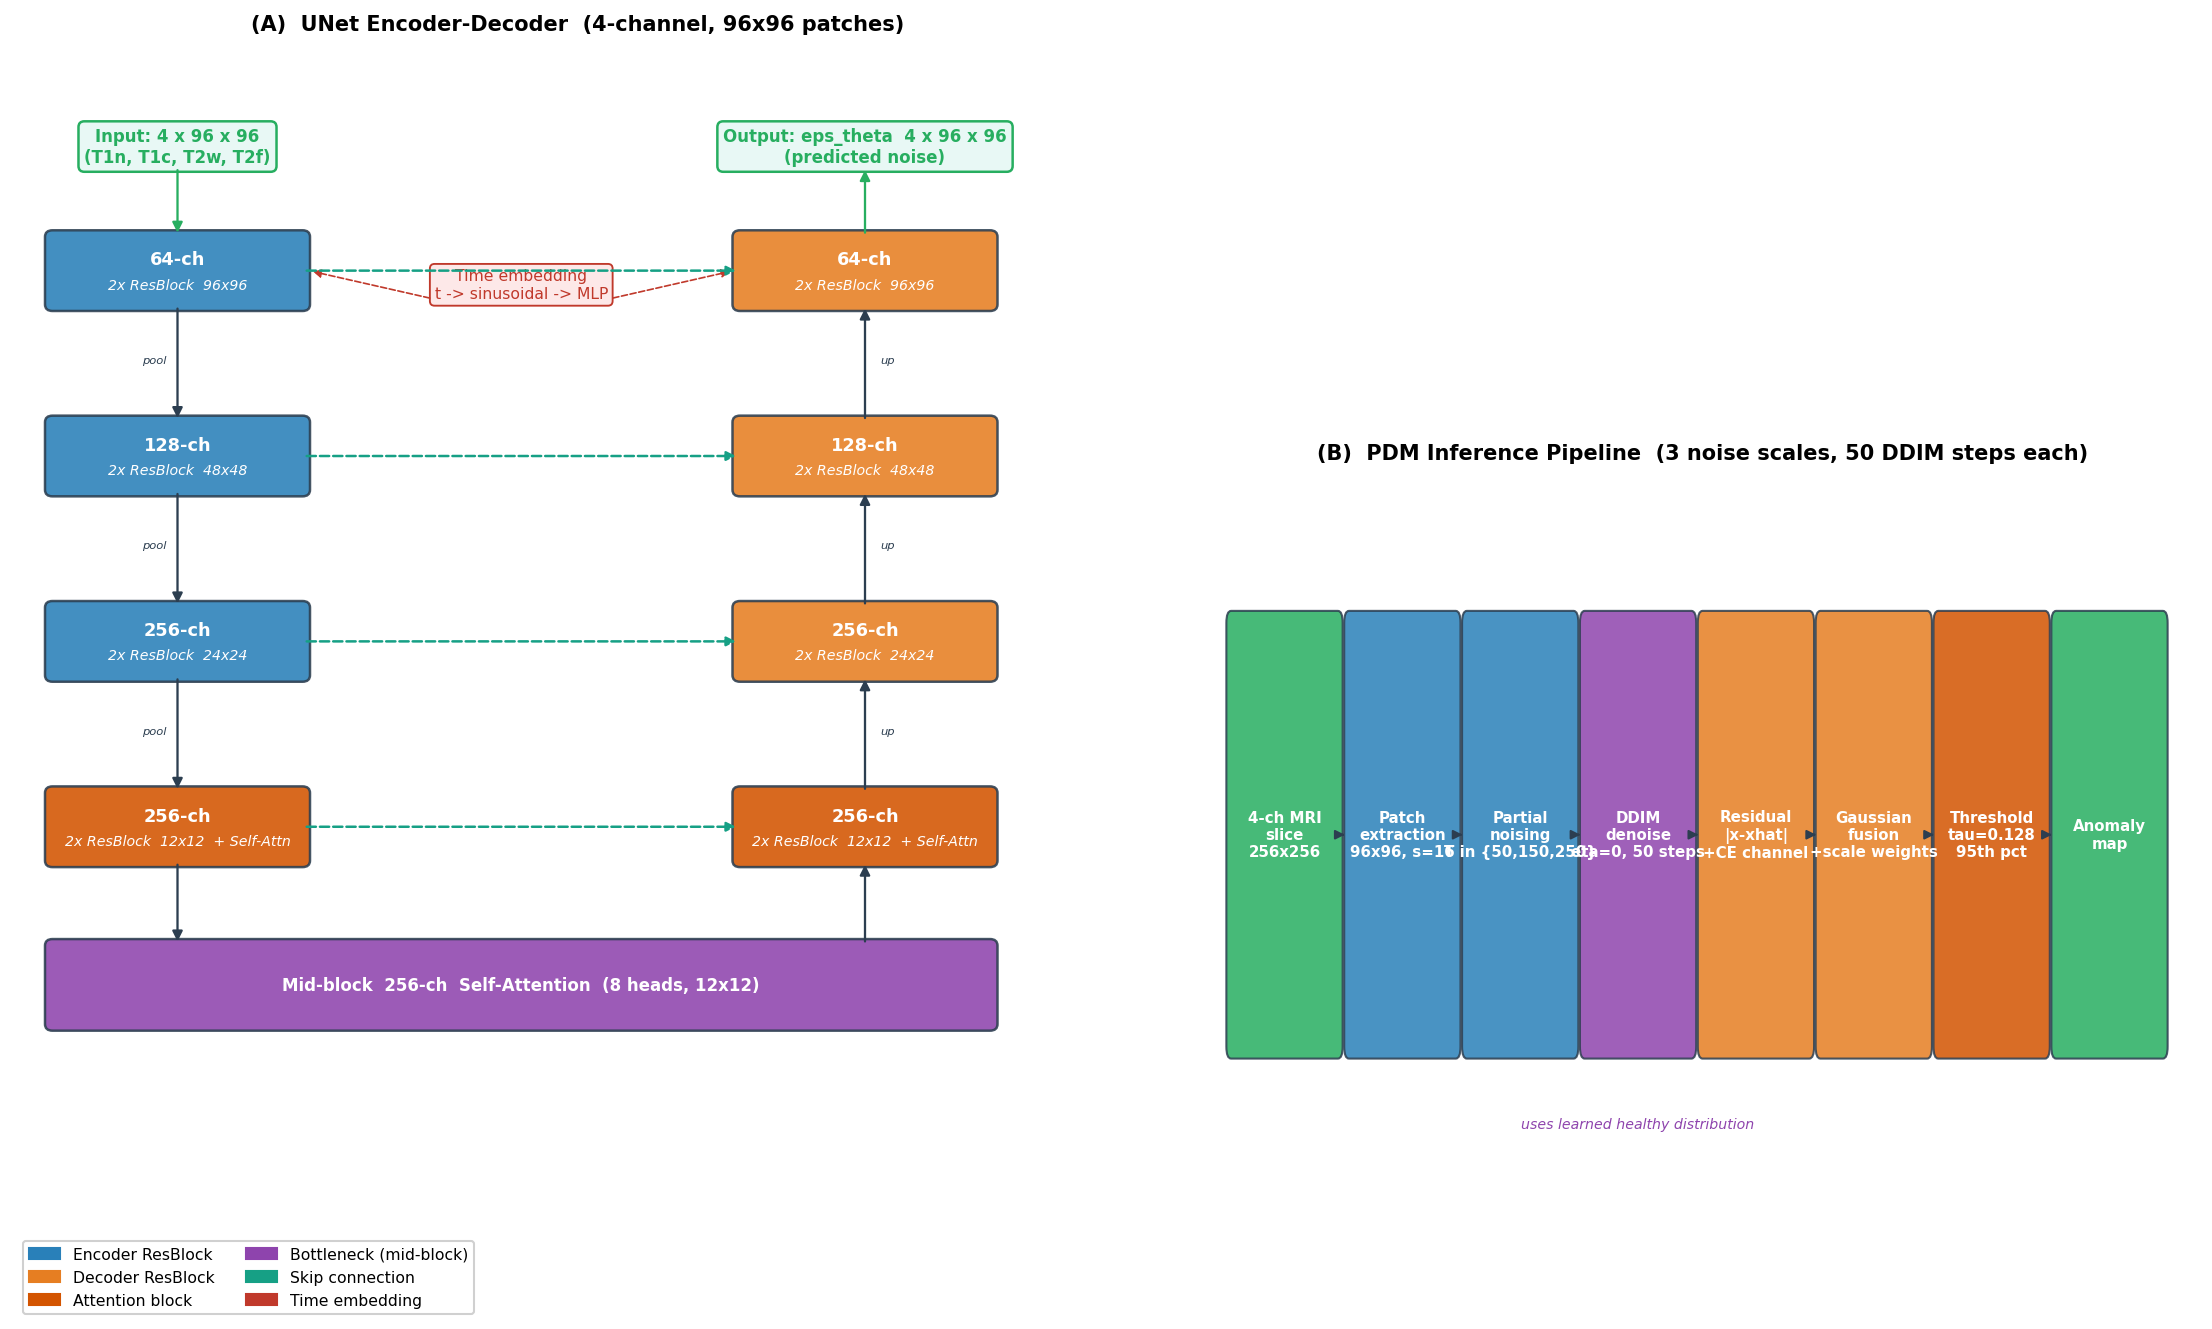
\includegraphics[width=\textwidth]{r-architecture.png}
\caption{(A) U-Net encoder-decoder architecture. The network operates on 4-channel
$96{\times}96$ patches. The encoder reduces spatial resolution from 96 to 12 pixels
across 4 levels (64, 128, 256, 256 channels). Self-attention is applied only at the
12${\times}$12 bottleneck (8 heads), keeping the model compact at 25.3\,M parameters.
Skip connections pass encoder features directly to the decoder at each level,
preserving fine detail in the reconstruction. The time embedding injects the
diffusion step $t$ into every residual block. (B) The full inference pipeline:
a test slice is cut into overlapping $96{\times}96$ patches, each is partially noised
and DDIM-denoised at three noise levels ($T\in\{50,150,250\}$), the residuals are
Gaussian-fused back into a full-slice map, scale weights combine the three maps, and
a threshold $\tau=0.128$ produces the final anomaly prediction.}
\label{fig:arch}
\end{figure}

\textbf{Calibration.} The threshold is the 95th percentile of pooled \emph{healthy}
brain-voxel scores, giving a controlled label-free false-positive rate; here
$\tau=0.128$.

% =====================================================================
\section{Training and Experimental Setup}
\label{sec:setup}
% =====================================================================

\subsection{Model configuration and hyperparameters}
Table~\ref{tab:hparams} lists all key settings used in this experiment.

\begin{table}[htbp]\centering\small
\caption{Model and training hyperparameters.}
\label{tab:hparams}
\begin{tabular}{@{}ll@{}}
\toprule
\textbf{Hyperparameter} & \textbf{Value} \\
\midrule
Patch size / stride & $96{\times}96$ / 16 px \\
U-Net block channels & $64 \to 128 \to 256 \to 256$ \\
U-Net parameters & 25.3\,M \\
Attention & 12${\times}$12 bottleneck only, 8 heads \\
Diffusion steps $T$ & 1000 (cosine schedule, $\beta\in[10^{-4},2{\times}10^{-2}]$) \\
Score timesteps & $\{50, 150, 250\}$ \\
Simplex noise & 6 octaves, persistence 0.8, lacunarity 2.0 \\
Batch size & $\approx$350 (effective) \\
Learning rate & $2{\times}10^{-4}$ (cosine decay, 1-epoch linear warmup) \\
Weight decay & $10^{-4}$ \\
EMA decay & 0.9999 \\
Gradient clip & 1.0 (global norm) \\
Calibration & 95th percentile of 200 healthy-slice pool \\
\bottomrule
\end{tabular}
\end{table}

The model used \textbf{bf16 automatic mixed precision} throughout. All reported numbers
use the \textbf{EMA weights}, not the raw weights; validation is also computed on the EMA
copy at the end of each epoch.

\paragraph{Validation protocol.} The validation loss is the same noise-prediction MSE as
training (Eq.~2), but measured on held-out \emph{healthy} patches from the validation
patients, with the EMA weights. The validation loader used 64 healthy slices (about
$7{,}700$ patches), kept fixed across epochs so the curve is comparable epoch to epoch.

\subsection{Compute budget and training duration}
Training ran on a single \textbf{NVIDIA A100 (80\,GB), Google Colab High-RAM}.
To keep each epoch within a fixed time budget, each epoch sampled a fixed
\textbf{250{,}000-patch} subset of the healthy pool (reshuffled each epoch), giving
\textbf{714 optimiser steps per epoch} (effective batch $\approx$350) and about
$9.4$\,min per epoch. The run was \textbf{scheduled for 60 epochs} ($\approx9.4$\,h
total) and reached its best validation loss at epoch 58. Early stopping (patience 6) did
not trigger, because the 60-epoch schedule ended before six epochs had passed without
improvement; the run was therefore stopped by the schedule, not by the early-stopping
rule. Evaluation covered 204 lesion slices from 4 test patients and took about
$92$\,s per slice (121 patches $\times$ three noise scales $\times$ 50 DDIM steps).

\begin{figure}[htbp]\centering
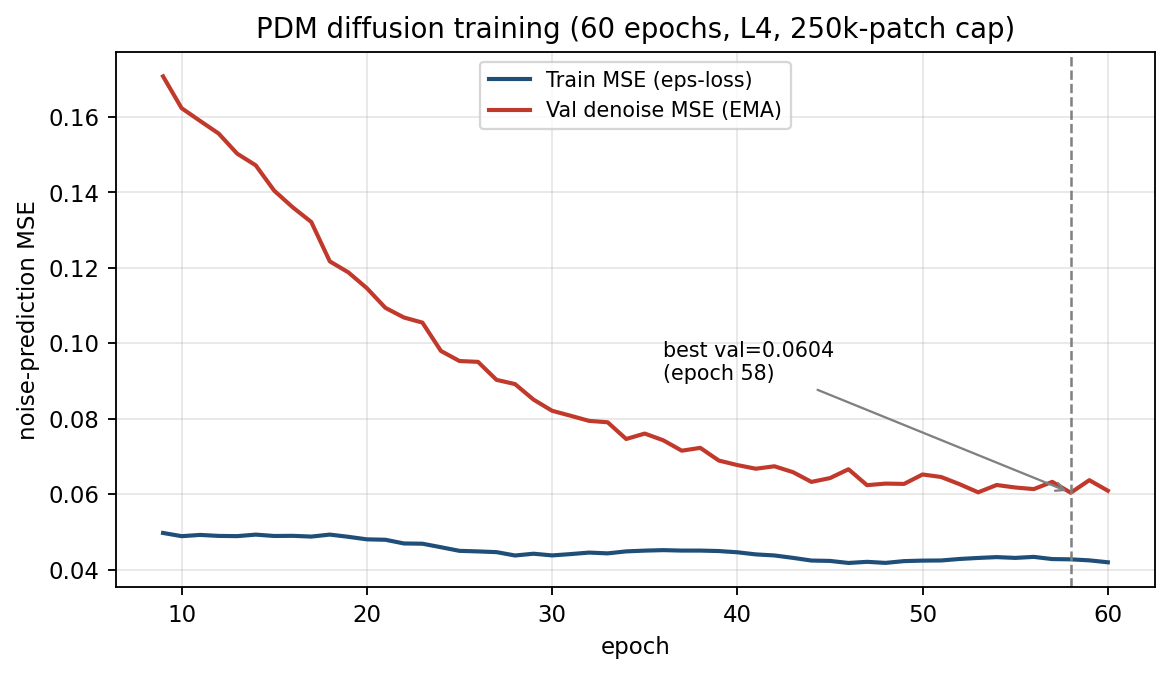
\includegraphics[width=0.72\textwidth]{r-training.png}
\caption{Diffusion training and validation noise-prediction MSE. The validation loss
(EMA weights) descends smoothly to a best of \textbf{0.0604 at epoch 58}; since the
noise has unit variance, this means the U-Net explains about \textbf{94\%} of the
injected-noise variance. Validation tracks training closely, with no upward divergence,
which indicates no over-fitting --- as expected given the large patch-level training set
(roughly $360{,}000$ patches, sampled at 250k per epoch).}
\label{fig:training}
\end{figure}

\begin{figure}[htbp]\centering
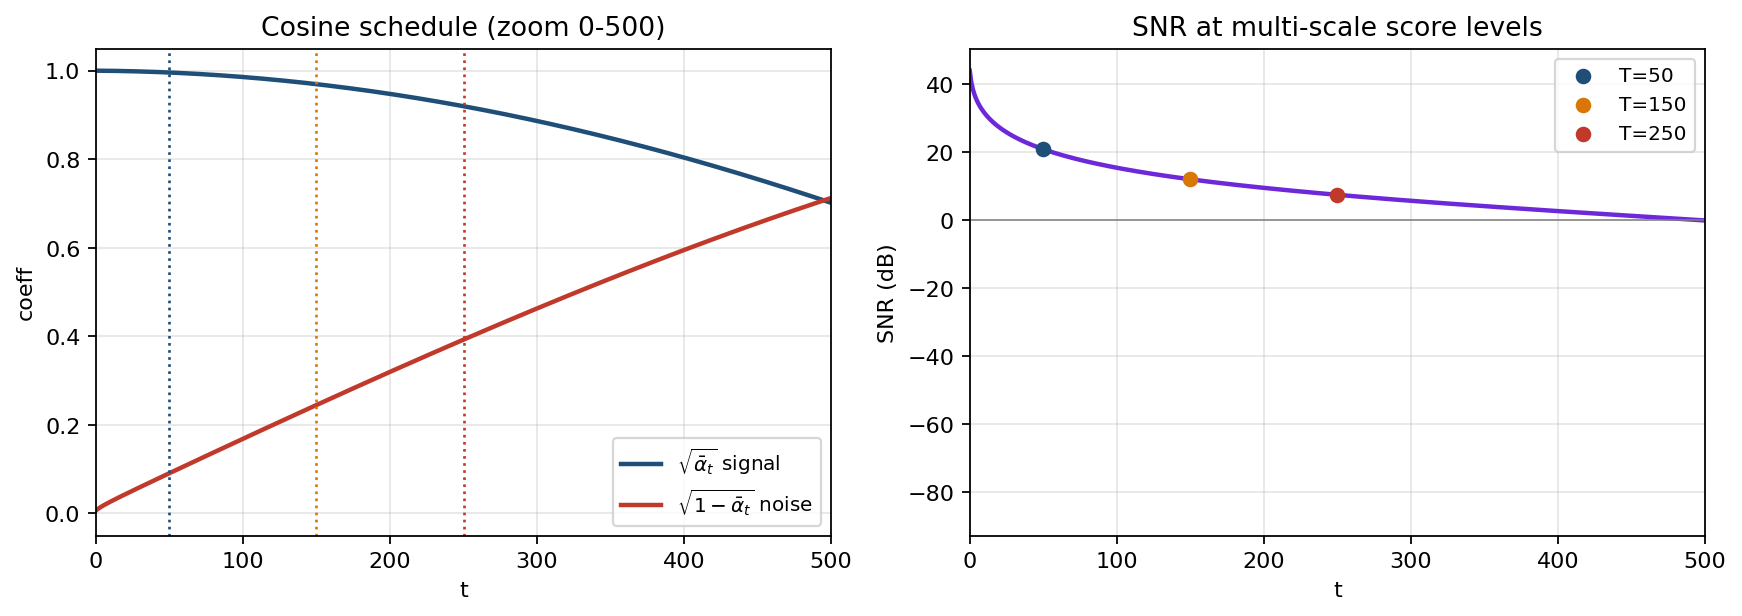
\includegraphics[width=0.92\textwidth]{r-schedule.png}
\caption{Cosine schedule and SNR. The multi-scale scoring levels correspond to
SNR $+20.8$\,dB ($T{=}50$, fine detail), $+11.9$\,dB ($T{=}150$), and $+7.4$\,dB
($T{=}250$, structural) --- progressively more aggressive ``healing''.}
\label{fig:schedule}
\end{figure}

% =====================================================================
\section{Results}
% =====================================================================
\subsection{Aggregate and per-patient performance}
Table~\ref{tab:results} reports metrics over the 204 evaluated test slices from 4 test
patients. The headline averages are AUROC $0.713$, AUPRC $0.076$, calibrated Dice
$0.076$, oracle Dice $0.138$. These numbers should be interpreted cautiously: four
patients is not enough to draw statistically reliable conclusions, and there are no
confidence intervals. The aggregate hides a strong bimodality: patient P00002 is
detected well (mean AUROC $0.893$), whereas P00216 fails (mean AUROC $0.571$, with
many slices below chance). One patient can shift the mean substantially in either
direction with this sample size.

\paragraph{How (un)reliable are these averages?} Across the four patients the spread is
large: the per-patient AUROC has a coefficient of variation of about $18\%$, and the
per-patient calibrated Dice about $130\%$ (driven by P00002 at $0.270$ against P00076 at
$0.013$). With $n=4$, only very large effects could be detected with any confidence, and
a single patient changes the mean appreciably. Bootstrap confidence intervals were not
computed; doing so over the 204 slices (resampling within patients) is listed as future
work (\S\ref{sec:future}). Until then, the headline averages should be read as
descriptive of these four patients, not as reliable population estimates.

\paragraph{Patient-mean vs.\ peak-slice (reconciling Tables \ref{tab:results} and
\ref{tab:lit}).} All numbers in Table~\ref{tab:results} are \emph{patient-level
means over every slice} --- e.g.\ P00002 is averaged across its 36 slices, giving
mean AUROC $0.893$ and mean calibrated Dice $0.270$. In contrast, the ``best
patient'' rows of Table~\ref{tab:lit} and the panels in Fig.~\ref{fig:perscale}
isolate the single \emph{peak slice} (P00002\,$z094$: AUROC $0.965$, AUPRC $0.533$,
fused Dice $0.589$). The per-slice peak is, by definition, higher than the 36-slice
mean, so the two tables are consistent --- they report different granularities, not
contradictory values.

\begin{table}[htbp]\centering
\caption{Per-patient and overall results (204 test slices). Dice at the calibrated
$\tau=0.128$; oracle = per-slice best threshold (upper bound).}
\label{tab:results}
\begin{tabular}{@{}lrcccc@{}}
\toprule
\textbf{Patient} & \textbf{Slices} & \textbf{AUROC} & \textbf{AUPRC} & \textbf{Dice (calib.)} & \textbf{Oracle Dice}\\
\midrule
P00203 & 61 & 0.750 & 0.047 & 0.053 & 0.108\\
\textbf{P00002} & 36 & \textbf{0.893} & \textbf{0.222} & \textbf{0.270} & \textbf{0.321}\\
P00216 & 53 & 0.571 & 0.039 & 0.035 & 0.073\\
P00076 & 54 & 0.692 & 0.046 & 0.013 & 0.112\\
\midrule
\textbf{Overall} & \textbf{204} & \textbf{0.713} & \textbf{0.076} & \textbf{0.076} & \textbf{0.138}\\
\bottomrule
\end{tabular}
\end{table}

\begin{figure}[htbp]\centering
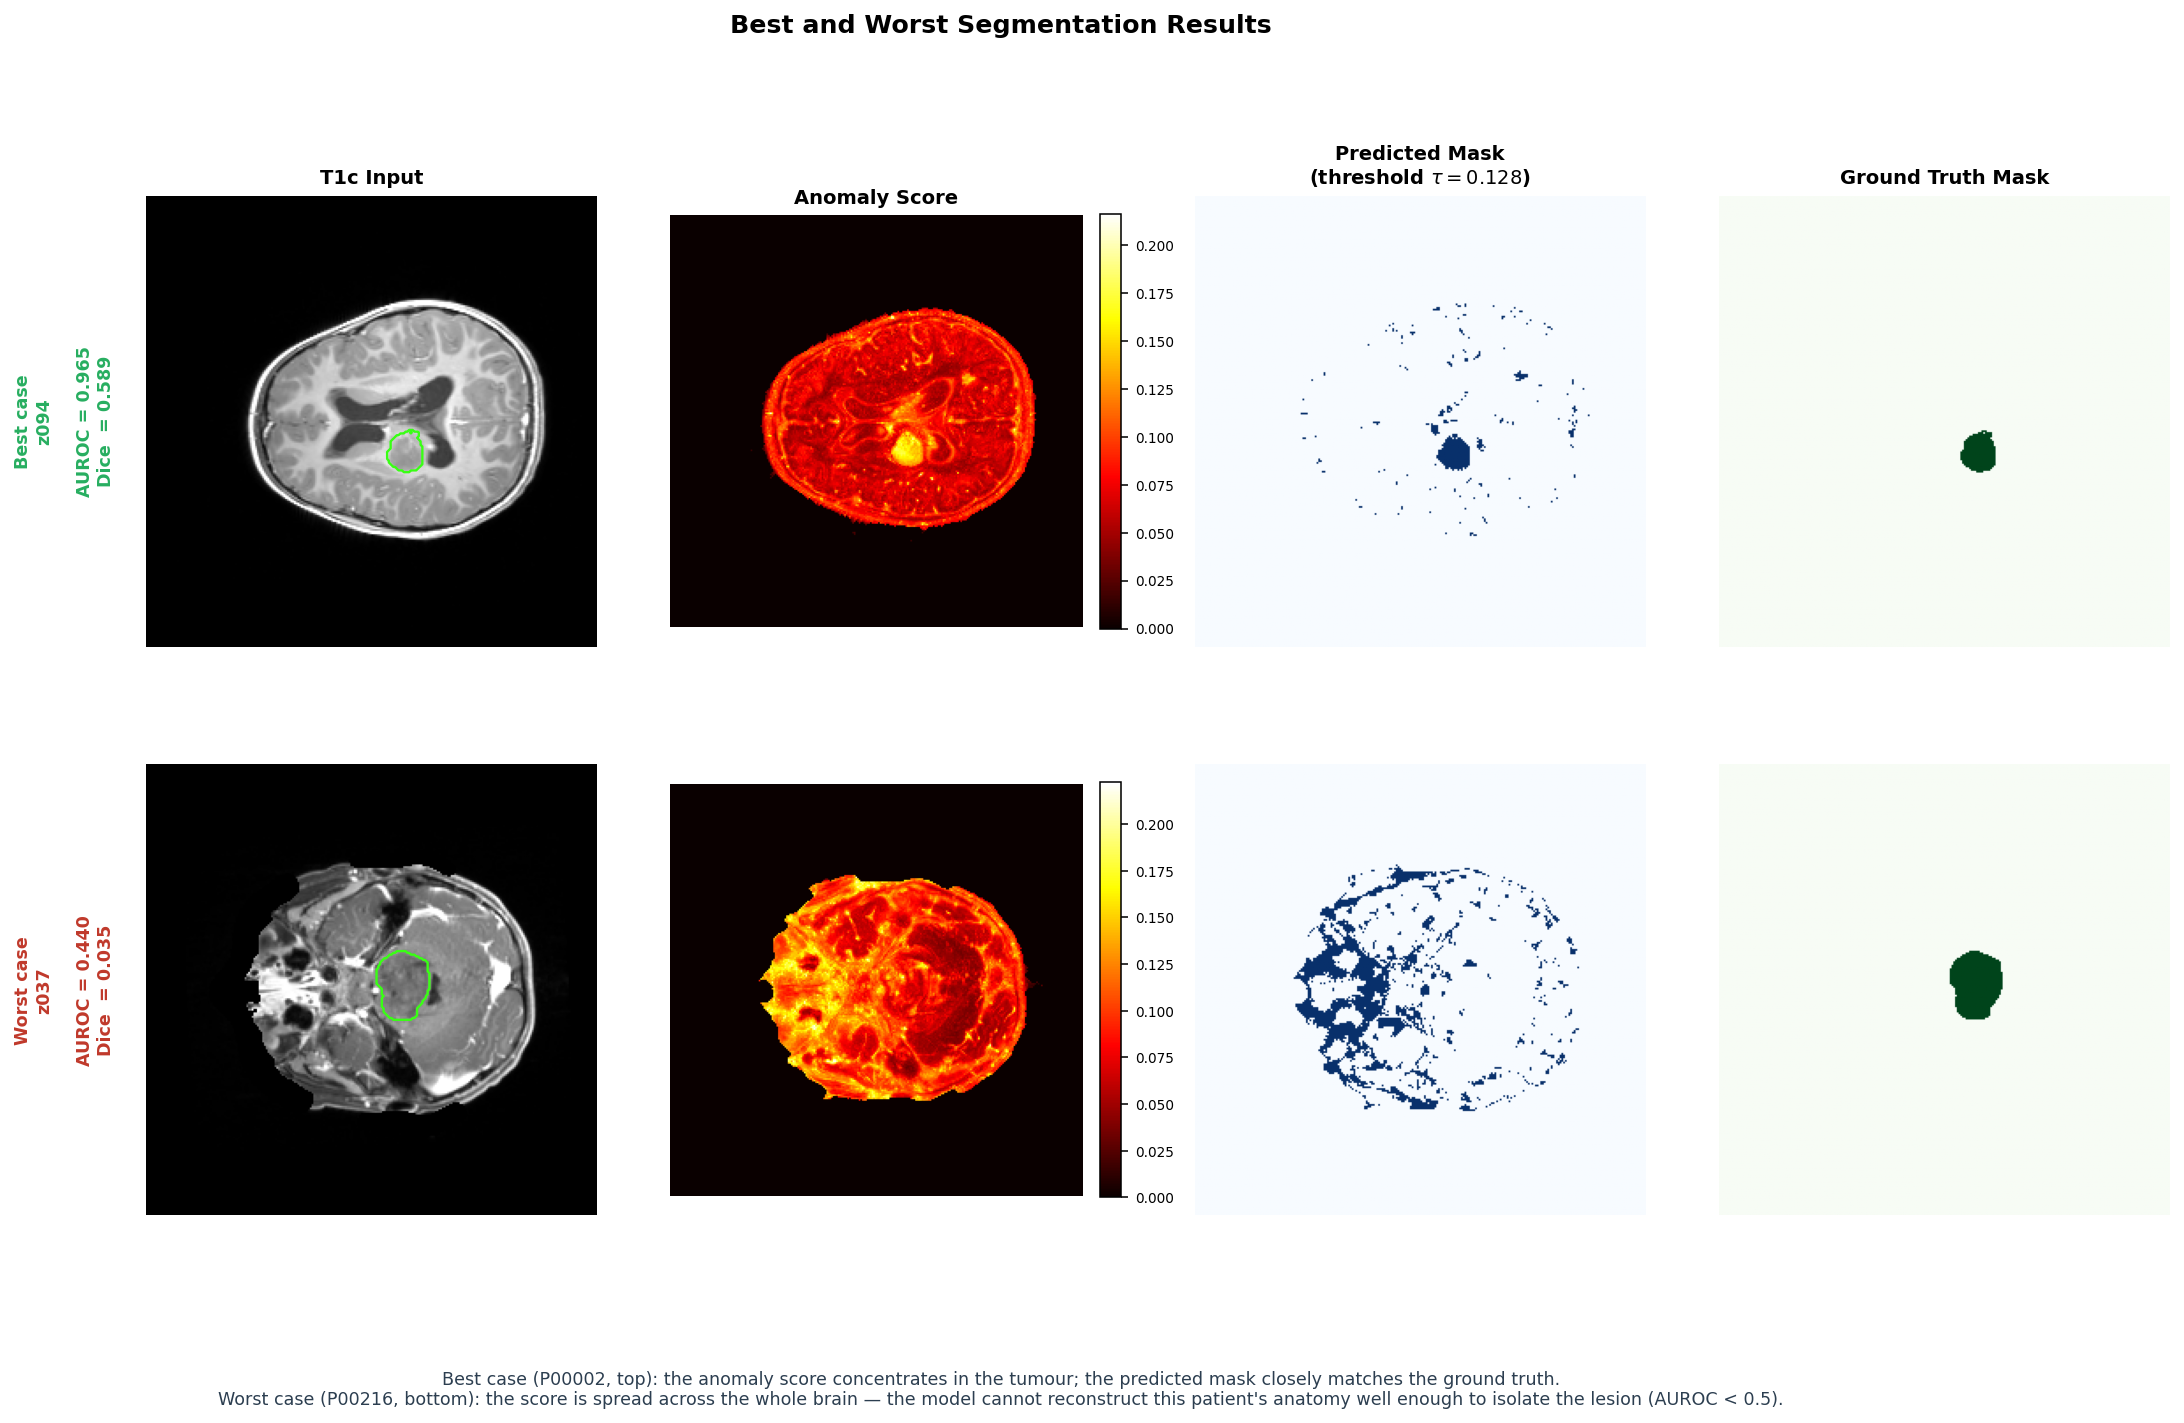
\includegraphics[width=\textwidth]{r-bestworst.png}
\caption{Best and worst segmentation results. \textbf{Top row} (P00002 $z094$,
AUROC 0.965, Dice 0.589): the anomaly score is concentrated inside the tumour
region; the predicted mask (at $\tau=0.128$) closely matches the ground truth.
\textbf{Bottom row} (P00216 $z037$, AUROC 0.440, Dice 0.035): the score is high
across the whole brain, not just the lesion --- the model cannot reconstruct this
patient's healthy tissue well enough to isolate the pathology. The same failure
mechanism is analysed quantitatively in \S\ref{sec:failure}.}
\label{fig:bestworst}
\end{figure}

\begin{figure}[htbp]\centering
\begin{subfigure}{0.49\textwidth}\centering
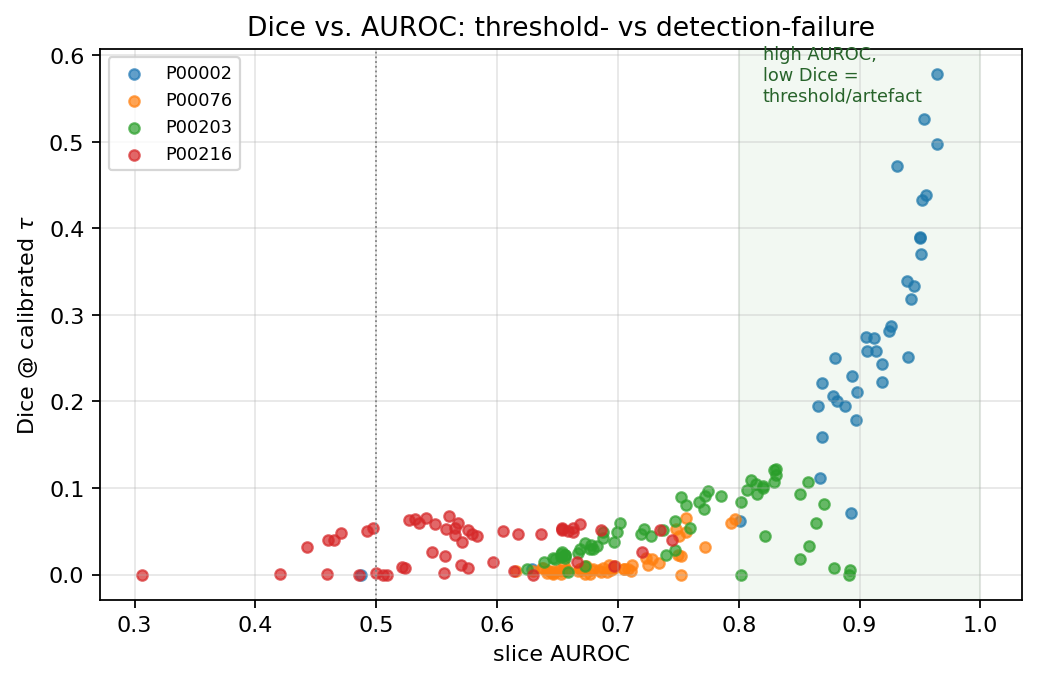
\includegraphics[width=\textwidth]{r-dice-auroc.png}\caption{Dice vs.\ AUROC}\label{fig:da}
\end{subfigure}\hfill
\begin{subfigure}{0.49\textwidth}\centering
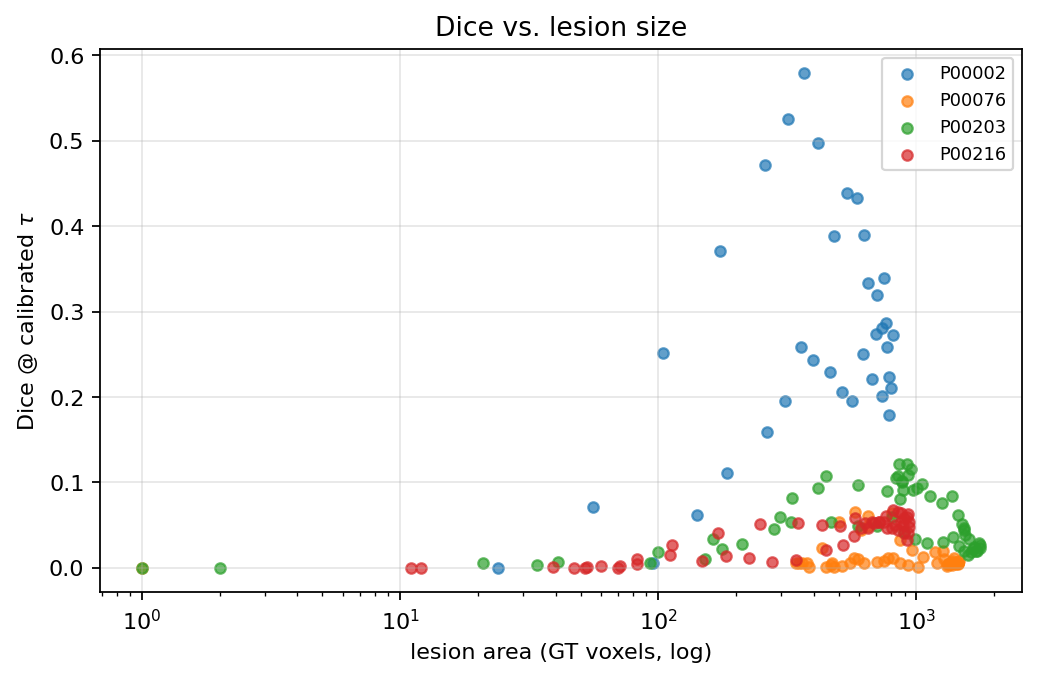
\includegraphics[width=\textwidth]{r-dice-area.png}\caption{Dice vs.\ lesion size}\label{fig:darea}
\end{subfigure}
\caption{Per-slice behaviour. (a) Patients separate into regimes: P00002 sits in the
high-AUROC/high-Dice zone; P00216 has many slices with \textbf{AUROC $<0.5$} (a
detection failure no threshold can fix). (b) Dice rises with lesion size --- small
lesions collapse precision (low AUPRC).}
\label{fig:scatters}
\end{figure}

\subsection{Training and validation behaviour}
The validation noise-MSE (Fig.~\ref{fig:training}) confirms a well-trained,
non-overfit denoiser: it decreases monotonically with the LR cycles and plateaus at
$0.0604$. This rules out under-training or over-fitting as explanations for the
downstream failures (\S\ref{sec:failure}).

% =====================================================================
\section{Failure Analysis: Why Does the Pilot Fail?}
\label{sec:failure}
% =====================================================================
This section uses figure-backed evidence to identify the most likely reason the
calibrated Dice is low, having already excluded data leakage (\S\ref{sec:leakage}),
under-training and over-fitting (Fig.~\ref{fig:training}). The analysis is based on
two diagnostic cases (one success, one failure), so the conclusions are
illustrative rather than statistically definitive.

\subsection{It is a score-separability problem, not a threshold problem}
Fig.~\ref{fig:hist} contrasts the per-voxel score distributions. For the success
slice (P00002 $z094$) the \emph{healthy} voxels peak at low scores ($\sim$0.05) and
the \emph{lesion} voxels peak high ($\sim$0.15): the two are well separated and the
calibrated $\tau=0.128$ sits cleanly between them, giving Dice $0.58$. For the
failure slice (P00216 $z037$) the healthy and lesion distributions are
\textbf{almost completely overlapping} --- the score simply does not distinguish
lesion from healthy tissue (slice AUROC $0.44$, below chance).

\begin{figure}[htbp]\centering
\begin{subfigure}{0.49\textwidth}\centering
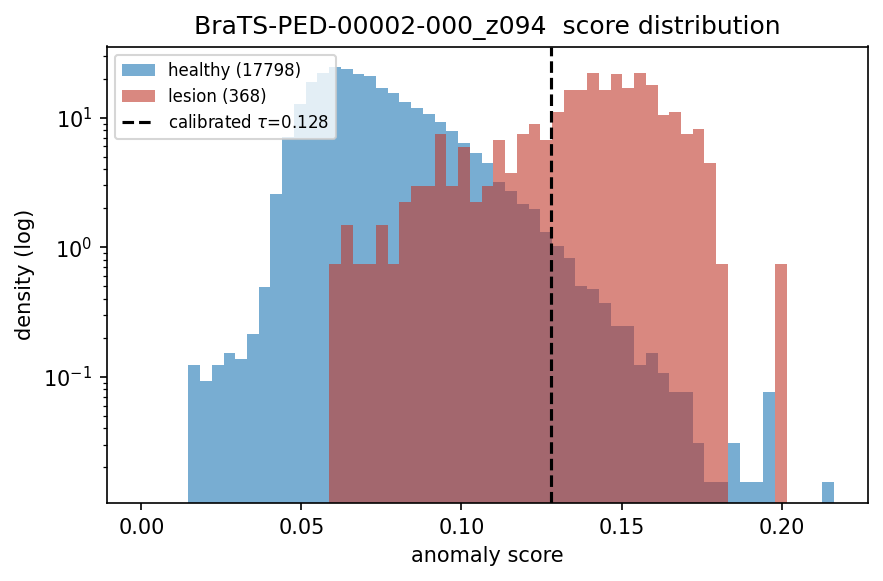
\includegraphics[width=\textwidth]{r-hist-success.png}\caption{Success (P00002\_z094)}\end{subfigure}\hfill
\begin{subfigure}{0.49\textwidth}\centering
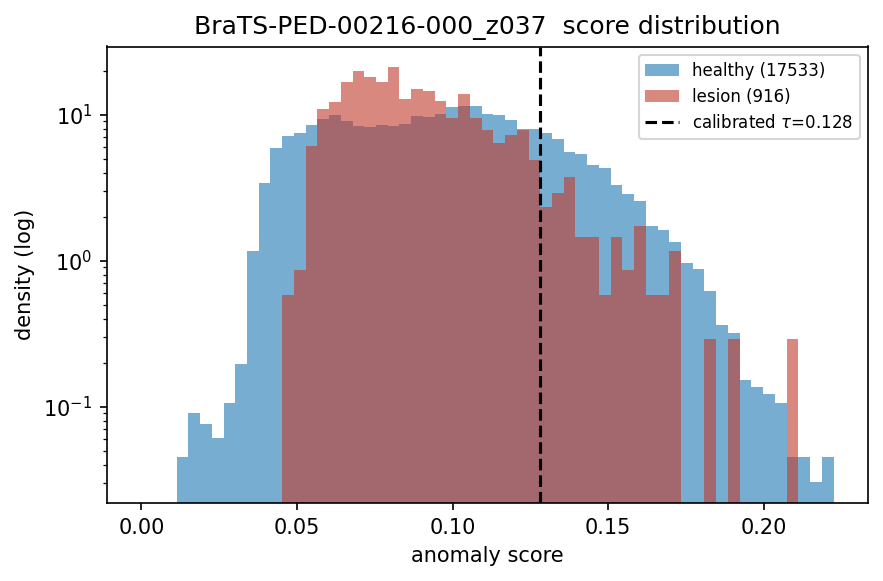
\includegraphics[width=\textwidth]{r-hist-failure.png}\caption{Failure (P00216\_z037)}\end{subfigure}
\caption{Healthy vs.\ lesion score distributions (log-density), with $\tau=0.128$.
Clean separation (left) vs.\ near-total overlap (right). The failure is an inability
of the \emph{score} to separate the classes.}
\label{fig:hist}
\end{figure}

Crucially, where detection works, the threshold itself is \textbf{not} the
bottleneck. Fig.~\ref{fig:thr} sweeps the threshold over the \emph{four diagnostic
slices} examined in this section (the two success and two failure cases above);
because this small sample is success-weighted, its absolute Dice ($\approx0.28$) is
far higher than the 204-slice corpus mean ($0.076$) and should not be read as a
corpus figure. The informative quantity is the curve's \emph{shape}: the calibrated
$\tau=0.128$ (mean Dice $0.284$) lies within $0.005$ Dice of the best global
threshold $\tau^\star=0.135$ (mean Dice $0.289$), i.e.\ the operating point is
near-optimal on slices where the score separates the classes. Corpus-wide, the
calibrated-to-oracle gap ($0.076\!\to\!0.138$, Table~\ref{tab:results}) shows a
single global threshold still leaves $\approx0.06$ Dice on the table across
heterogeneous slices --- a secondary lever --- but the dominant failure (P00216,
slice AUROC $<0.5$) is \emph{threshold-independent}: no threshold recovers a score
that does not rank lesion above healthy tissue.

\begin{figure}[htbp]\centering
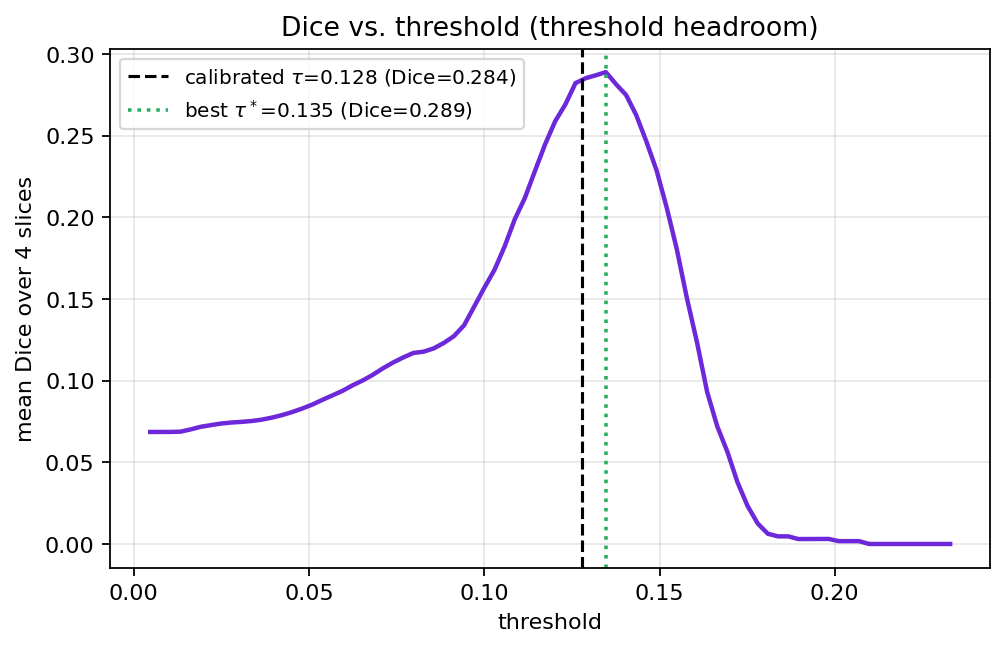
\includegraphics[width=0.6\textwidth]{r-dice-threshold.png}
\caption{Mean Dice vs.\ threshold over the \emph{four diagnostic slices} of this
section. These are a success-weighted sample (two success, two failure), so absolute
Dice values ($\approx0.28$) are much higher than the 204-slice corpus mean ($0.076$)
--- this figure is about \emph{shape}, not level. The calibrated $\tau$ (black)
falls within $0.005$ Dice of the sweep optimum (green) on these slices, suggesting
that on cases where the score already separates the classes, the threshold adds
little extra error. This does not imply the threshold is optimal corpus-wide.}
\label{fig:thr}
\end{figure}

\subsection{Root cause: per-patient reconstruction fidelity / out-of-manifold anatomy}
Why can the score separate lesions on P00002 but not P00216?
Fig.~\ref{fig:maskedge} shows that on the failure patient the anomaly score is high
across the \emph{entire} brain parenchyma --- not the lesion --- and
Fig.~\ref{fig:modres} shows the per-modality residual is diffuse across all
modalities, not localised. The model reconstructs this patient's \emph{healthy}
tissue poorly, so every voxel has a large residual and the lesion contrast vanishes.
The most plausible reading, given this evidence, is that P00216's anatomy \textbf{appears
out-of-distribution} for the healthy manifold learned from only 30 training patients: the
residual then measures distance from the training manifold, which is uniformly large,
rather than local pathology. P00002, whose anatomy is better represented and whose tumour
is a compact contrast-enhancing mass, yields the intended localised residual. This is a
hypothesis consistent with the figures, not a proven cause (see the threats to validity
below).

\begin{figure}[htbp]\centering
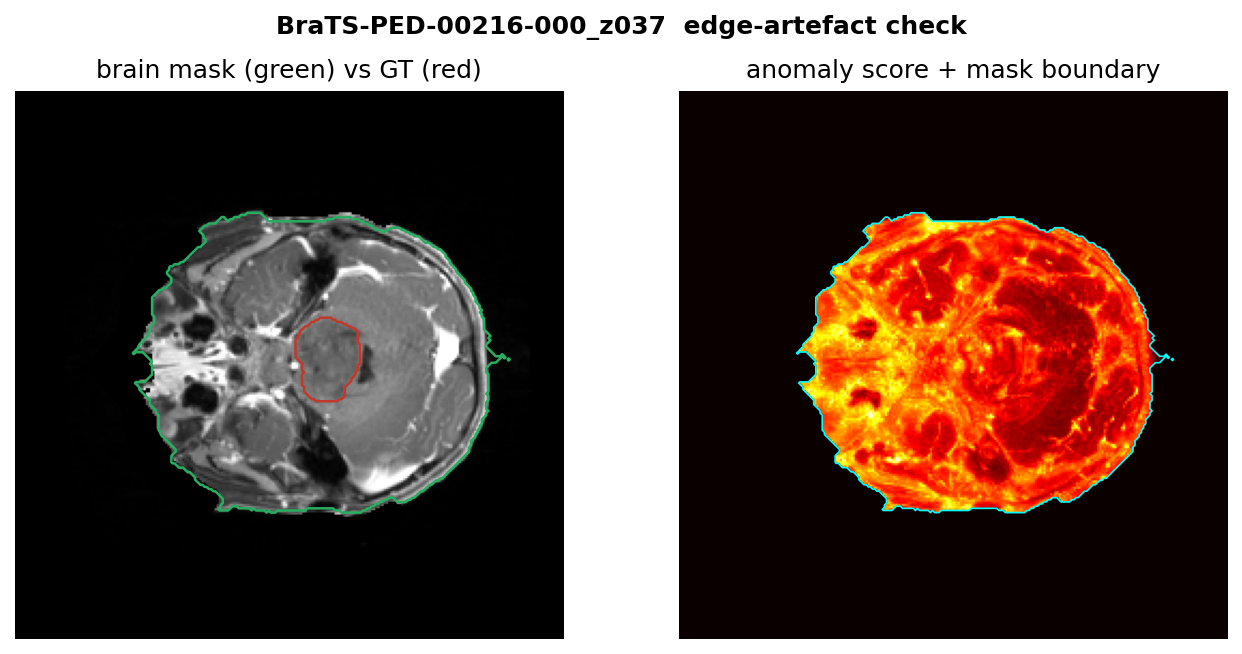
\includegraphics[width=0.78\textwidth]{r-maskedge-failure.png}
\caption{Failure (P00216\_z037): the brain mask (green) is correct and the GT lesion
(red) is a small central mass, yet the anomaly score (right) is high over the
\emph{whole} parenchyma. The residual reflects global reconstruction error, not the
lesion.}
\label{fig:maskedge}
\end{figure}

\begin{figure}[htbp]\centering
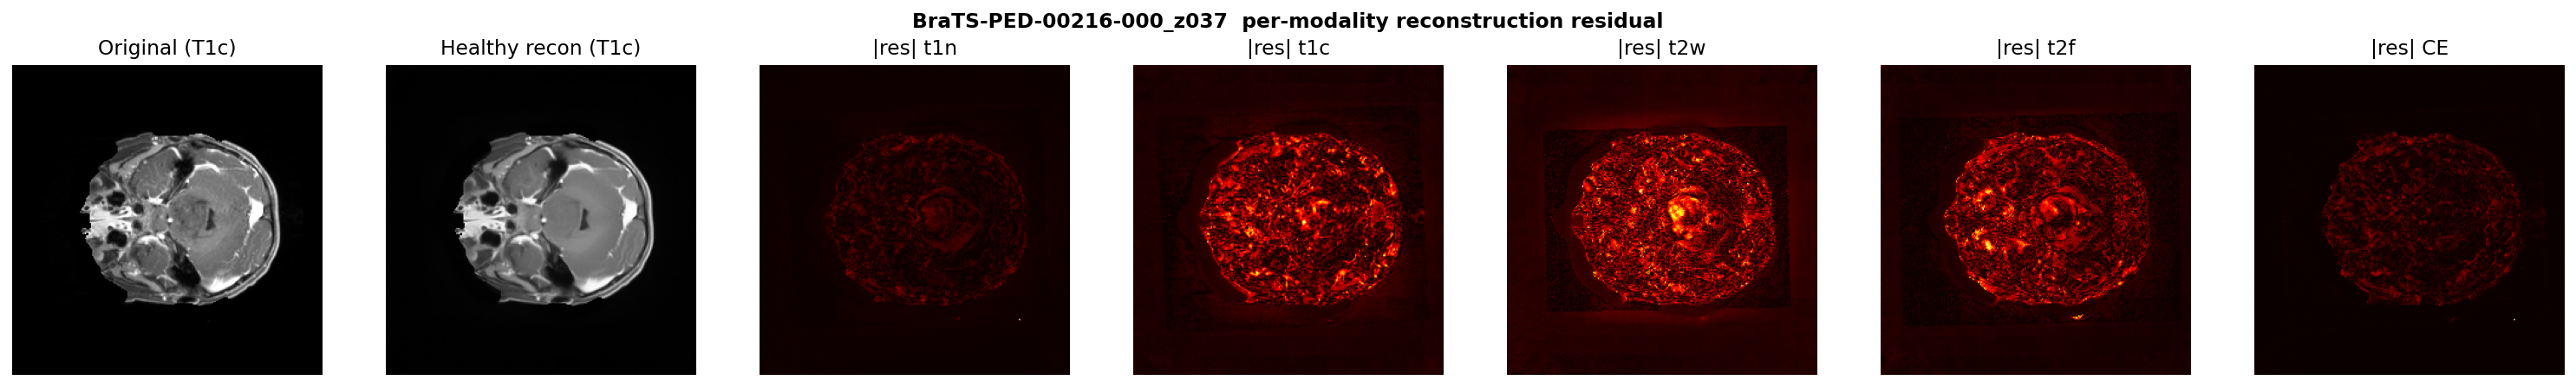
\includegraphics[width=\textwidth]{r-modres-failure.png}
\caption{Per-modality reconstruction residual for the failure slice. The error is
diffuse across $t1c$, $t2w$, $t2f$ (not localised to the lesion), confirming a
whole-slice reconstruction-fidelity failure rather than a scoring-weight issue.}
\label{fig:modres}
\end{figure}

\subsection{Two distinct, separable failure modes}
The per-slice scatter (Fig.~\ref{fig:da}) makes the taxonomy explicit:
\begin{enumerate}[leftmargin=1.5em,itemsep=1pt]
\item \textbf{Detection failure} (P00216): slice AUROC $\le0.5$. The score ranks
lesion voxels no better than (sometimes worse than) healthy ones. \emph{No}
threshold recovers it (oracle Dice also low, $0.073$). Cause: OOD anatomy / poor
healthy reconstruction.
\item \textbf{Precision / small-lesion failure} (P00076, parts of P00203): AUROC is
respectable ($0.65$--$0.78$) but Dice and AUPRC are low because the lesion is small
relative to a diffuse low-level false-positive field, so precision collapses.
\end{enumerate}
The most plausible shared explanation for both failure modes is the same: the training
set is probably too small to cover all the healthy anatomy types in the test set, so the
model cannot reconstruct every patient faithfully. This is presented as the leading
hypothesis, not a settled conclusion.

\subsection{Threats to validity}
Because the analysis rests on four test patients and two diagnostic slices, several
alternative explanations cannot be ruled out. They are listed here honestly:
\begin{itemize}[leftmargin=1.4em,itemsep=1pt]
\item \textbf{Confounded patient factors.} P00216 may differ from P00002 in tumour type,
size, location, patient age, or acquisition protocol. Any of these could drive the poor
reconstruction independently of training-set coverage; with $n=4$ these cannot be
separated.
\item \textbf{Acquisition / preprocessing artefacts.} A different scanner, contrast
protocol, or a registration or normalisation artefact specific to P00216 could also
produce a diffuse residual.
\item \textbf{No dose-response evidence.} It has not been shown that adding training
patients actually improves reconstruction on patients like P00216; that link is assumed,
not demonstrated.
\end{itemize}
The proper test of the training-size hypothesis is the scaling experiment in
\S\ref{sec:future}. Until then, this section is best read as \emph{hypothesis
generation}: it identifies a plausible and falsifiable cause and the experiment that
would confirm or refute it.

\subsection{Candidate causes that appear unlikely (given available evidence)}
For each of the following, there is evidence suggesting it is \emph{not} the primary
cause --- though a definitive ruling-out would require a controlled experiment:
data leakage (\S\ref{sec:leakage}, patient-level splits + label-free training);
under-training / over-fitting (Fig.~\ref{fig:training}, smooth converged val loss);
threshold miscalibration (Fig.~\ref{fig:thr}, $\tau$ within $0.005$ Dice of
the sweep optimum on the four examined slices); and scoring-weight error
(Fig.~\ref{fig:modres}, residual is diffuse in \emph{every} modality, so
re-weighting alone cannot localise it).

% =====================================================================
\section{Explainability (XAI) and Inference Behaviour}
\label{sec:xai}
% =====================================================================
\subsection{Why post-hoc saliency is the wrong tool here}
A natural first instinct is to apply Grad-CAM \cite{selvaraju2017} for a ``where did
the model look'' map. This is \emph{unfaithful} for a generative diffusion UAD model:
Grad-CAM localises the regions that raise a single \emph{class logit}, but a
denoiser has no class head. The only available scalar is the dense-regression noise
error, whose global-average-pooled gradient collapses all spatial information into a
per-channel weight, leaving the map with no spatial selectivity. Empirically it is
diffuse \emph{even on slices where the anomaly score sharply localises the lesion}
(Fig.~\ref{fig:xai}, top-right was such a failed map) --- failing the sanity
criterion that an explanation track the model's output \cite{adebayo2018} and the
faithfulness requirement for high-stakes use \cite{rudin2019}. Post-hoc CAM is therefore
rejected in favour of explainers \emph{intrinsic} to the decision.

\subsection{Faithful explainers for this pipeline}
\textbf{(i) Counterfactual generation (primary).} The healthy reconstruction
$\hat\x$ \emph{is} the thresholded decision variable, so $|\x-\hat\x|$ is faithful by
construction (no surrogate), and $\hat\x$ is the projection of the patient onto the
healthy manifold/prototype (Appendix~\ref{app:math}, Eq.~\eqref{eq:prototype})
\cite{wachter2017,sanchez2022,wolleb2022}. Fig.~\ref{fig:xai} shows it isolates a
sharp tumour hot-spot on the success slice and is diffuse on the failure slice ---
\emph{visually predicting the metric outcome without the ground truth}.
\textbf{(ii) Residual attribution (supporting).} Because the score is an
\emph{exact additive} sum over modalities and scales, attribution is exact:
Fig.~\ref{fig:attr} decomposes the score by modality, showing FLAIR ($t2f$)
dominates the genuine lesion (success) while the failure case spreads more evenly
across modalities --- the signature of a whole-brain reconstruction error rather
than localised pathology. \textbf{(iii) Per-scale / partial-diffusion}
(Fig.~\ref{fig:attr}b) shows each noise level's contribution; for compact tumours
the higher-SNR scales localise best. Together these turn each prediction into a
checkable statement and \emph{flag the failures} (diffuse counterfactual + even
modality split) label-free.

\begin{figure}[htbp]\centering
\begin{subfigure}{\textwidth}\centering
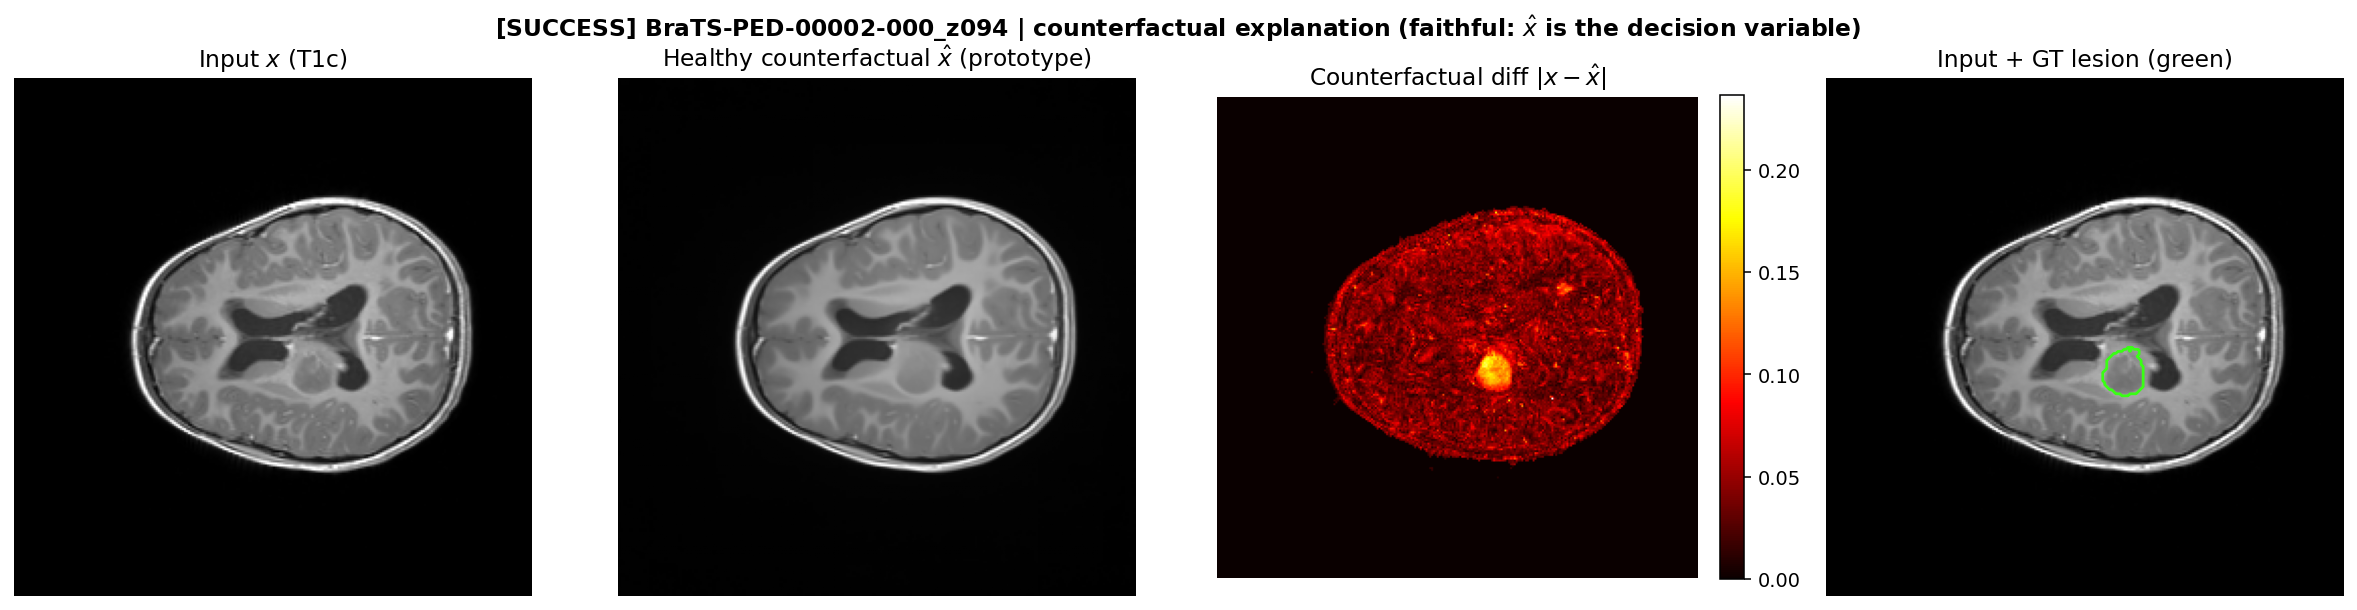
\includegraphics[width=0.92\textwidth]{r-counterfactual-success.png}\caption{Success (P00002\,$z094$): the counterfactual difference is a sharp tumour hot-spot.}\end{subfigure}\\[4pt]
\begin{subfigure}{\textwidth}\centering
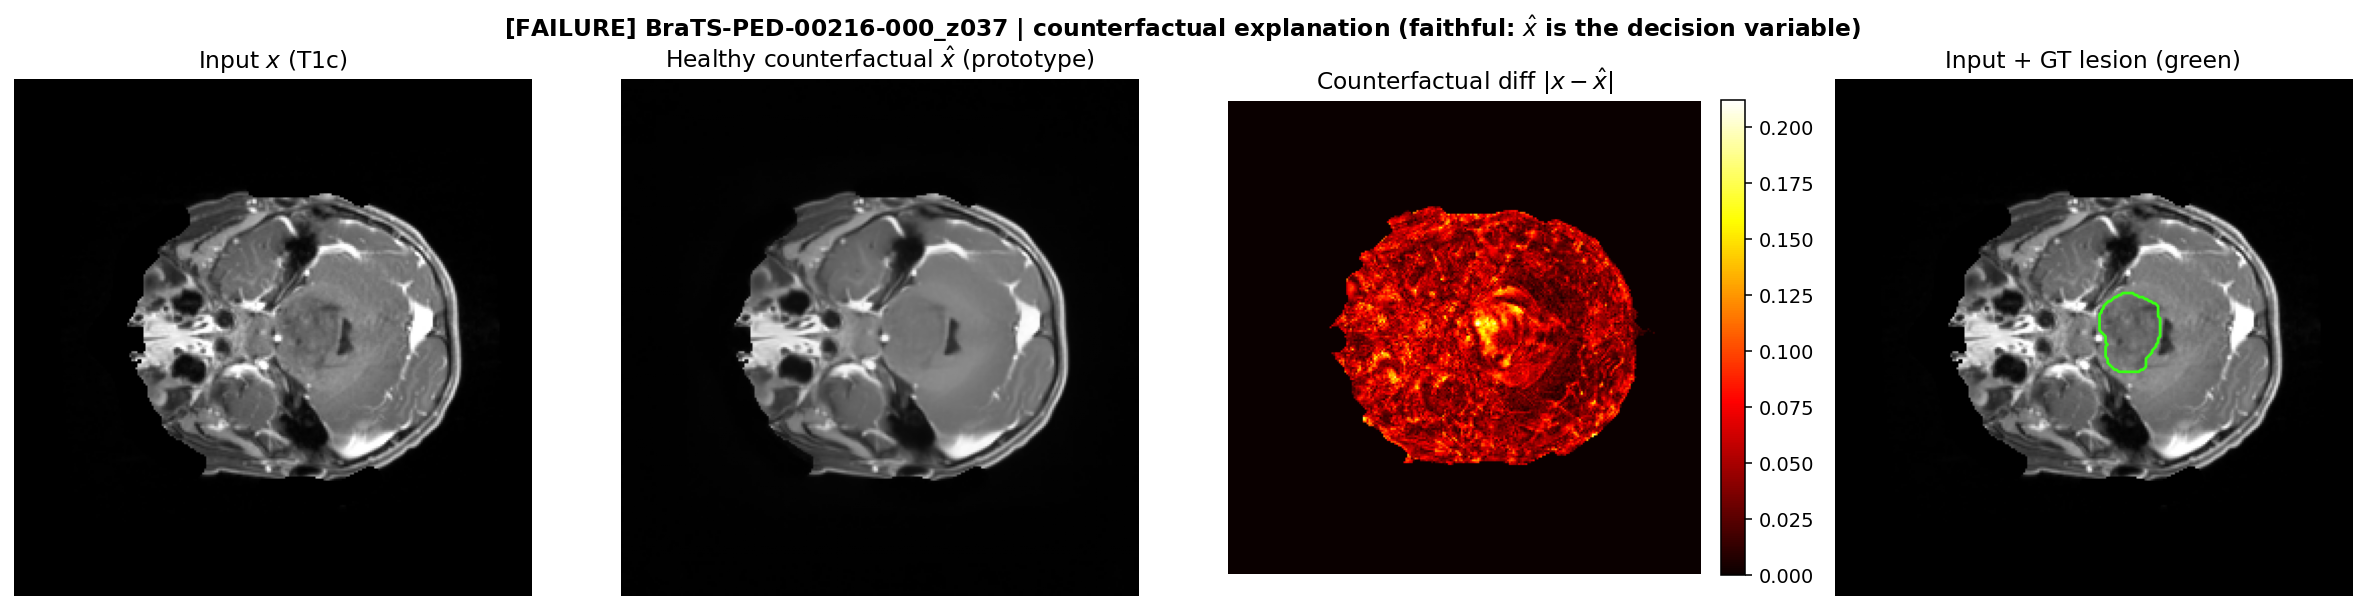
\includegraphics[width=0.92\textwidth]{r-counterfactual-failure.png}\caption{Failure (P00216\,$z037$): the counterfactual is diffuse over the whole parenchyma.}\end{subfigure}
\caption{Counterfactual explanation (the faithful primary explainer): input $\x$,
healthy prototype $\hat\x$, difference $|\x-\hat\x|$, and the GT lesion. It localises
on the success slice and is diffuse on the failure slice --- predicting the outcome
without labels, which the (rejected) Grad-CAM map could not do.}
\label{fig:xai}
\end{figure}

\begin{figure}[htbp]\centering
\begin{subfigure}{0.46\textwidth}\centering
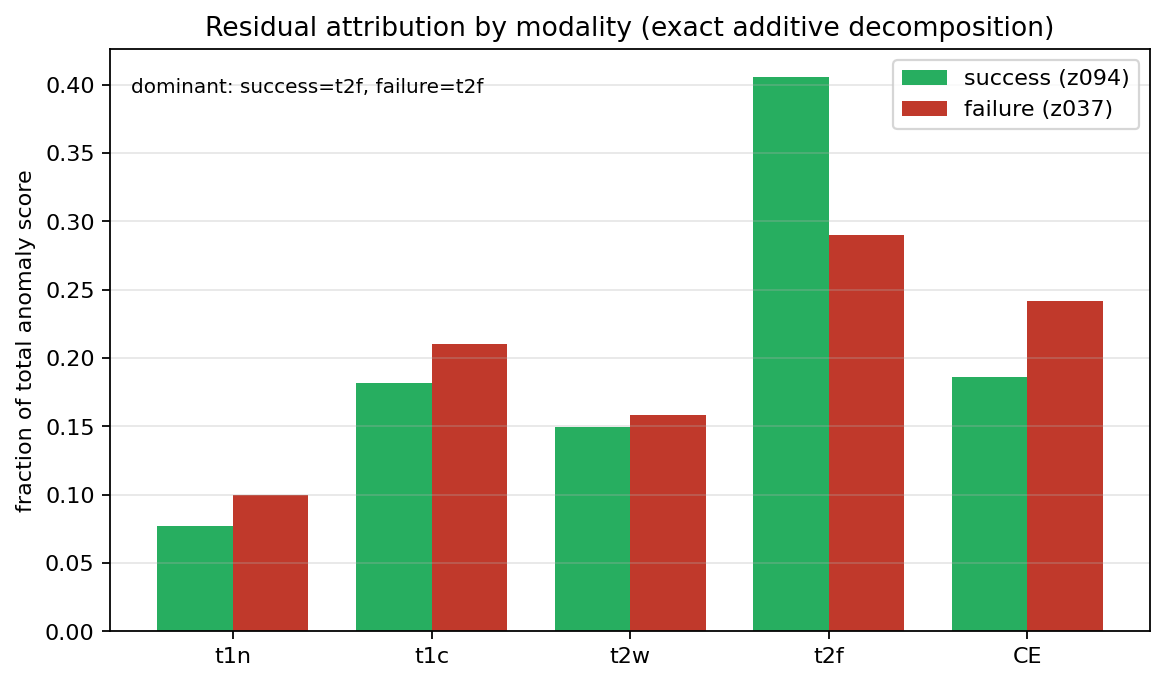
\includegraphics[width=\textwidth]{r-residual-attribution.png}\caption{Residual attribution by modality}\end{subfigure}\hfill
\begin{subfigure}{0.52\textwidth}\centering
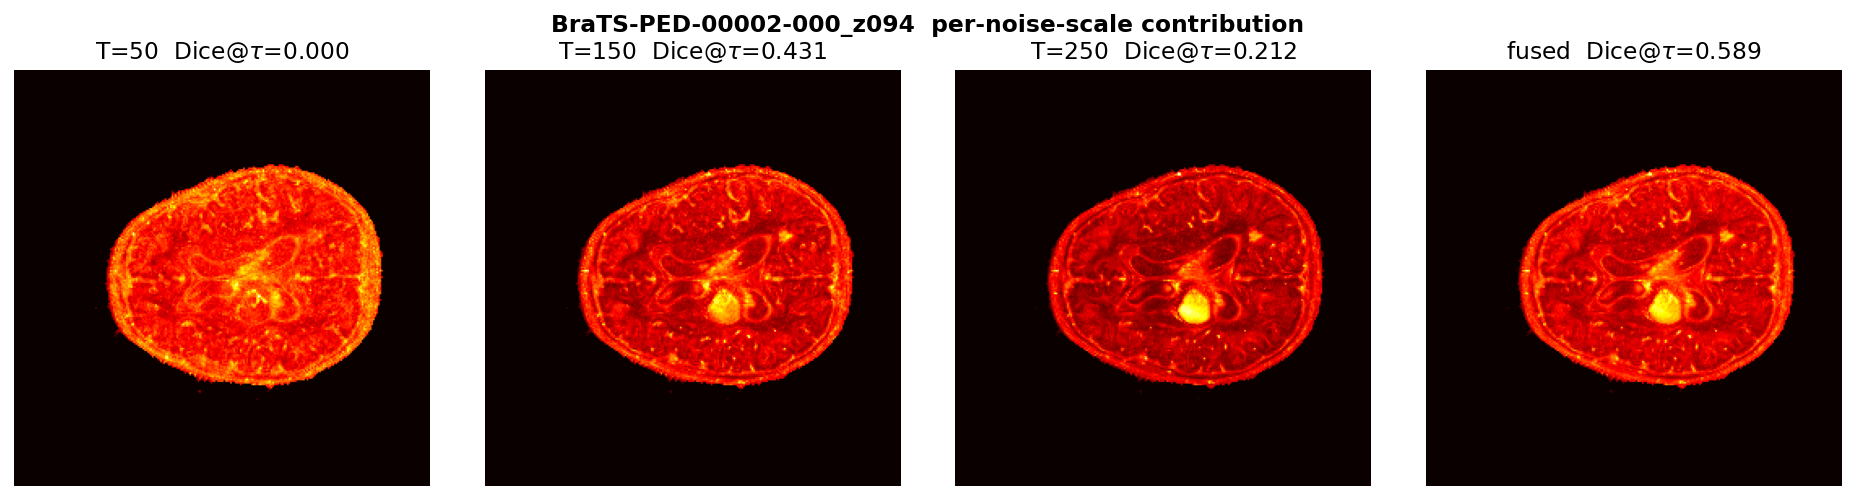
\includegraphics[width=\textwidth]{r-perscale-success.png}\caption{Per-scale maps + Dice@$\tau$ (P00002\,$z094$)}\end{subfigure}
\caption{Exact additive attribution. (a) By modality: FLAIR ($t2f$) dominates the
genuine lesion (success) while the failure spreads across modalities. (b) By noise
scale (partial diffusion): higher-SNR scales localise the compact tumour.}
\label{fig:attr}
\end{figure}

\begin{figure}[htbp]\centering
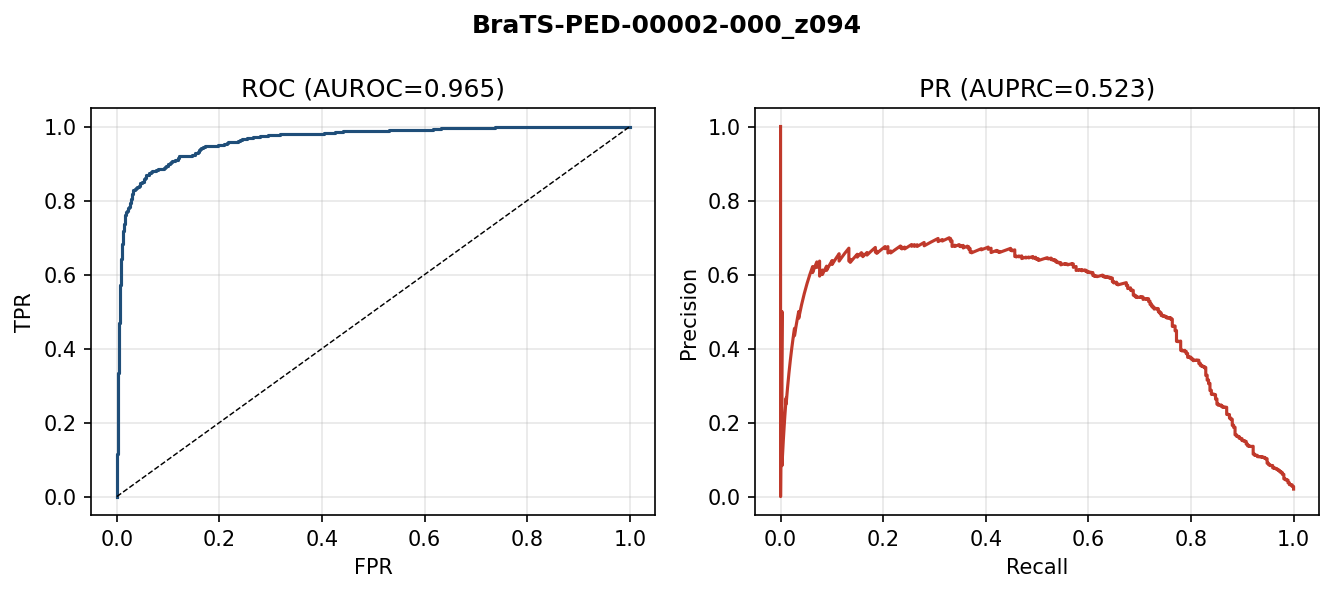
\includegraphics[width=0.5\textwidth]{r-rocpr-success.png}
\caption{ROC / PR curves underlying the success slice (P00002\,$z094$, AUROC
$0.965$).}
\label{fig:perscale}
\end{figure}

% =====================================================================
\section{Comparison with the Literature}
% =====================================================================
Table~\ref{tab:lit} places this work's numbers next to representative reconstruction-based
UAD results. Three caveats are essential for an honest reading: (1) the cited works
are on \emph{adult} BraTS, which is larger and less anatomically variable than
BraTS-PEDs; (2) they use \emph{full} training cohorts, versus the 30-patient pilot here;
(3) several report best/oracle-style Dice, which corresponds to the oracle column here,
not the calibrated column. The fair comparison is therefore the \emph{oracle} and
\emph{best-slice} figures of this work against their reported Dice.

\begin{table}[htbp]\centering\small
\caption{Reconstruction-based UAD on BraTS (as reported). Numbers are indicative;
datasets/protocols differ (see caveats). $^\dagger$ adult BraTS.}
\label{tab:lit}
\begin{tabularx}{\textwidth}{@{}lll cc X@{}}
\toprule
\textbf{Method} & \textbf{Backbone} & \textbf{Dice} & \textbf{AUROC} & \textbf{AUPRC} & \textbf{Notes}\\
\midrule
f-AnoGAN \cite{schlegl2019}      & GAN            & $\sim$0.24 & $\sim$0.86 & --- & adult$^\dagger$, full\\
AE/VAE comp.\ \cite{baur2021}    & Autoencoders   & 0.31--0.37 & 0.80--0.90 & --- & adult$^\dagger$, full\\
AnoDDPM \cite{wyatt2022}         & DDPM+simplex   & $\sim$0.44 & --- & --- & adult$^\dagger$, full\\
pDDPM \cite{behrendt2023}        & Patch DDPM     & $\sim$0.49 & --- & --- & adult$^\dagger$, full\\
Wolleb \cite{wolleb2022}         & Guided diff.   & $\sim$0.60 & --- & --- & weak guidance\\
\midrule
\textbf{This work} --- calibrated avg   & Patch DDPM     & 0.076 & 0.713 & 0.076 & \textbf{pediatric, 30-pt pilot, 204 sl}\\
\textbf{This work} --- oracle avg       & Patch DDPM     & 0.138 & 0.713 & 0.076 & per-slice best $\tau$\\
\textbf{This work} --- best slice (P00002 $z094$) & Patch DDPM  & \textbf{0.589} & \textbf{0.965} & 0.533 & peak slice (not patient mean)\\
\bottomrule
\end{tabularx}
\end{table}

\textbf{How should this comparison be read?} The results are mixed and the comparison
must be made carefully. On its best slice (P00002\,$z094$) the method reaches Dice
$0.589$ / AUROC $0.965$, which is \emph{in the range of} what methods trained on full
adult cohorts report \cite{wyatt2022,behrendt2023,wolleb2022}. But three differences make
this far from a like-for-like result: those methods evaluate on adult BraTS with hundreds
to roughly a thousand patients, not a single pediatric slice; Wolleb et al.
\cite{wolleb2022} (Dice $\approx0.60$) is \emph{weakly supervised} via classifier
guidance, whereas this work uses no labels; and a single peak slice is not a patient or
cohort average. The pilot \emph{average} here (Dice $0.076$, AUROC $0.713$) is clearly
below the literature, and it would be wrong to call the method ``competitive'' on the
strength of one good patient out of four. No confidence intervals are reported, so even
these numbers carry unknown error bars. The failure analysis suggests the gap is driven by
out-of-manifold patients under the 30-patient training budget --- a data-coverage problem
--- but, as §\ref{sec:failure} stresses, that rests on two diagnostic cases and would need
the controlled scaling experiment (30 vs.\ 60 vs.\ 180 patients) to be confirmed. The
likely headroom is in training scale and reconstruction fidelity, both directly
addressable (\S\ref{sec:future}).

% =====================================================================
\section{Limitations and Future Work}
\label{sec:future}
% =====================================================================
\textbf{Limitations.}

\textit{Dataset size.} The training set is only 30 patients, which is not enough to
cover the full range of healthy pediatric brain anatomy. The test set is only 4
patients (204 slices). With such a small sample, one patient dominates the average
(P00002 alone accounts for most of the oracle Dice), and the results have no
statistical reliability. No confidence intervals or bootstrap estimates are reported.
Any conclusion beyond ``this case worked / this case did not'' should be treated with
caution until evaluated on a larger cohort.

\textit{No ablation studies.} The pipeline combines several components --- simplex
noise, patch diffusion, Gaussian fusion, multi-scale scoring, modality weighting, the
CE channel, and DDIM reconstruction. No ablation table is provided. It is therefore
not possible to say which components actually help and by how much. Patch diffusion
and simplex noise are inherited from prior work \cite{behrendt2023,wyatt2022} and
have individual ablations in those papers, but the specific combination used here has
not been tested systematically.

\textit{No hyperparameter sensitivity analysis.} The modality weights, score timesteps
$T\in\{50,150,250\}$, and calibration threshold are set by hand or by a single-pass
sweep. Whether small changes to these values affect the results significantly is
unknown.

\textit{XAI evaluation is qualitative.} The counterfactual and residual-attribution
explanations are assessed visually on two example slices. No quantitative XAI metrics
(insertion/deletion curves, pointing game, faithfulness scores) are reported. The
qualitative evidence is consistent with the score maps, but formal evaluation is
needed before drawing strong conclusions about the explanations.

\textit{Boundary artefacts.} The residual is slightly elevated near the brain
boundary. A global threshold does not distinguish this from genuine lesion signal,
which reduces precision on small peripheral lesions.

\textbf{Future work.}
(1) \textbf{Full-cohort training} on the full 180-patient BraTS-PEDs training split ---
this is the single most important step; without it, the failure-analysis conclusions
remain hypotheses.
(2) \textbf{Ablation study} to isolate the contribution of each component.
(3) \textbf{Scaling experiment} (30 $\to$ 60 $\to$ 180 patients) to confirm that
broader healthy-manifold coverage is the dominant lever, and to quantify the
improvement per added patient.
(4) \textbf{Reconstruction quality gate}: automatically flag patients whose global
residual is too high for reliable scoring, converting silent failures into abstentions.
(5) \textbf{Per-slice adaptive thresholding} to close the calibrated-to-oracle Dice
gap on precision-limited patients.
(6) \textbf{Quantitative XAI evaluation} with insertion/deletion or pointing-game
metrics to put the counterfactual explanations on a formal footing.
(7) \textbf{Boundary-aware masking} to reduce false positives near the skull rim.
(8) \textbf{Attention-rollout maps} (Abnar \& Zuidema, 2020): the U-Net's
self-attention at the $12{\times}12$ bottleneck could be traced back to patch
positions to give a model-internal complement to the counterfactual explanation.
The config flag \texttt{attention\_rollout} is wired; only the visualisation script
is missing.

% =====================================================================
\section{Conclusion}
% =====================================================================
This project built and evaluated a patch-diffusion UAD pipeline for pediatric brain MRI,
with a faithful explainability layer and careful controls against data leakage. The
diffusion model trains well (validation noise-MSE $0.0604$) and, on its best-represented
patient, reaches Dice $0.58$ and AUROC $0.96$. The pilot average (Dice $0.076$, AUROC
$0.713$) is below the literature. The failure analysis --- based on two illustrative
cases --- \emph{generates the hypothesis} that the leading cause is per-patient
reconstruction fidelity rather than a flaw in the detector itself, and the confounders
this small sample cannot rule out have been stated explicitly. On slices where the score
already separates the two classes, the calibrated threshold is near-optimal. The clearest
next step is full-cohort training to broaden healthy-manifold coverage, together with the
scaling experiment that would actually test the hypothesis. As a 30-patient proof of
concept, the work runs end-to-end, the failure modes are clearly characterised, and the
path to improvement is concrete and falsifiable.

% =====================================================================
\begin{thebibliography}{99}
\small
\bibitem{ho2020} Ho, J., Jain, A., Abbeel, P. (2020). \textit{Denoising Diffusion Probabilistic Models}. NeurIPS.
\bibitem{song2021} Song, J., Meng, C., Ermon, S. (2021). \textit{Denoising Diffusion Implicit Models}. ICLR.
\bibitem{nichol2021} Nichol, A., Dhariwal, P. (2021). \textit{Improved Denoising Diffusion Probabilistic Models}. ICML.
\bibitem{rombach2022} Rombach, R., et al. (2022). \textit{High-Resolution Image Synthesis with Latent Diffusion Models}. CVPR.
\bibitem{wyatt2022} Wyatt, J., et al. (2022). \textit{AnoDDPM: Anomaly Detection with DDPMs using Simplex Noise}. CVPR-W.
\bibitem{behrendt2023} Behrendt, F., et al. (2023). \textit{Patched Diffusion Models for Unsupervised Anomaly Detection in Brain MRI}. MIDL. arXiv:2303.03758.
\bibitem{bercea2023} Bercea, C., et al. (2023). \textit{Generalizing Unsupervised Anomaly Detection}. MICCAI.
\bibitem{graham2023} Graham, M., et al. (2023). \textit{Denoising Diffusion Models for OOD Detection}. CVPR-W.
\bibitem{wolleb2022} Wolleb, J., et al. (2022). \textit{Diffusion Models for Medical Anomaly Detection}. MICCAI.
\bibitem{pinaya2022} Pinaya, W., et al. (2022). \textit{Fast Unsupervised Brain Anomaly Detection with Latent Diffusion Models}. MICCAI.
\bibitem{baur2021} Baur, C., et al. (2021). \textit{Autoencoders for Unsupervised Anomaly Segmentation in Brain MR Images: A Comparative Study}. Medical Image Analysis.
\bibitem{schlegl2019} Schlegl, T., et al. (2019). \textit{f-AnoGAN}. Medical Image Analysis.
\bibitem{zimmerer2022} Zimmerer, D., et al. (2022). \textit{Medical Out-of-Distribution Analysis Challenge}. IEEE TMI.
\bibitem{kazerooni2024} Kazerooni, A. F., et al. (2024). \textit{BraTS Challenge 2023: Focus on Pediatrics (BraTS-PEDs)}. arXiv:2305.17033.
\bibitem{menze2015} Menze, B., et al. (2015). \textit{The Multimodal Brain Tumor Image Segmentation Benchmark (BRATS)}. IEEE TMI.
\bibitem{selvaraju2017} Selvaraju, R., et al. (2017). \textit{Grad-CAM: Visual Explanations from Deep Networks via Gradient-based Localization}. ICCV.
\bibitem{adebayo2018} Adebayo, J., et al. (2018). \textit{Sanity Checks for Saliency Maps}. NeurIPS.
\bibitem{rudin2019} Rudin, C. (2019). \textit{Stop Explaining Black Box Machine Learning Models for High-Stakes Decisions and Use Interpretable Models Instead}. Nature Machine Intelligence.
\bibitem{wachter2017} Wachter, S., et al. (2017). \textit{Counterfactual Explanations without Opening the Black Box}. Harvard JOLT.
\bibitem{sanchez2022} Sanchez, P., et al. (2022). \textit{Healthy/Pathological Brain Counterfactuals with Diffusion Models}. arXiv:2203.08089.
\bibitem{wang2003} Wang, Z., et al. (2003). \textit{Multiscale Structural Similarity}. Asilomar.
\bibitem{ronneberger2015} Ronneberger, O., et al. (2015). \textit{U-Net}. MICCAI.
\bibitem{kascenas2023} Kascenas, A., et al. (2023). \textit{The Role of Noise in Denoising Models for Anomaly Detection in Brain MRI}. Medical Image Analysis.
\bibitem{kawar2022} Kawar, B., et al. (2022). \textit{Denoising Diffusion Restoration Models}. NeurIPS.
\bibitem{chung2023} Chung, H., et al. (2023). \textit{Diffusion Posterior Sampling for General Noisy Inverse Problems}. ICLR.
\end{thebibliography}

% =====================================================================
\appendix
\section{Complete Mathematical Derivation}
\label{app:math}
The following is the full, self-contained derivation of the DDPM/DDIM machinery and
the PDM scoring used above (forward kernel, variational bound, posterior,
$\eps$-objective, DDIM, simplex noise, patch fusion, multi-scale scoring,
calibration, metrics, and the counterfactual / residual-attribution mathematics).
\bigskip
\input{math_body.tex}

\end{document}
